%%%%%%%%%%%%%%%%%%%%%%%%%%%%%%%%%%%%%%%%%
% Beamer Presentation
% LaTeX Template
% Version 1.0 (10/11/12)
%
% This template has been downloaded from:
% http://www.LaTeXTemplates.com
%
% License:
% CC BY-NC-SA 3.0 (http://creativecommons.org/licenses/by-nc-sa/3.0/)
%
%%%%%%%%%%%%%%%%%%%%%%%%%%%%%%%%%%%%%%%%%

%----------------------------------------------------------------------------------------
%	PACKAGES AND THEMES
%----------------------------------------------------------------------------------------

\documentclass[aspectratio=32]{beamer}
\usefonttheme[onlymath]{serif}


\mode<presentation> {

% The Beamer class comes with a number of default slide themes
% which change the colors and layouts of slides. Below this is a list
% of all the themes, uncomment each in turn to see what they look like.

\usetheme{default}
%\usetheme{AnnArbor}
%\usetheme{Antibes}
%\usetheme{Bergen}
%\usetheme{Berkeley}
%\usetheme{Berlin}
%\usetheme{Boadilla}
%\usetheme{CambridgeUS}
%\usetheme{Copenhagen}
%\usetheme{Darmstadt}
%\usetheme{Dresden}
%\usetheme{Frankfurt}
%\usetheme{Goettingen}
%\usetheme{Hannover}
%\usetheme{Ilmenau}
%\usetheme{JuanLesPins}
%\usetheme{Luebeck}
%\usetheme{Malmoe}
%\usetheme{Marburg}
%\usetheme{Montpellier}
%\usetheme{PaloAlto}
%\usetheme{Pittsburgh}
%\usetheme{Rochester}
%\usetheme{Singapore}
%\usetheme{Szeged}
%\usetheme{Warsaw}

% As well as themes, the Beamer class has a number of color themes
% for any slide theme. Uncomment each of these in turn to see how it
% changes the colors of your current slide theme.

%\usecolortheme{albatross}
%\usecolortheme{beaver}
\usecolortheme{spruce}
%\usecolortheme{beetle}
%\usecolortheme{crane}
%\usecolortheme{dolphin}
%\usecolortheme{dove}
%\usecolortheme{fly}
%\usecolortheme{lily}
%\usecolortheme{orchid}
%\usecolortheme{rose}
%\usecolortheme{seagull}
%\usecolortheme{seahorse}
%\usecolortheme{whale}
%\usecolortheme{wolverine}

%\setbeamertemplate{footline} % To remove the footer line in all slides uncomment this line
%\setbeamertemplate{footline}[page number] % To replace the footer line in all slides with a simple slide count uncomment this line

%\setbeamertemplate{navigation symbols}{} % To remove the navigation symbols from the bottom of all slides uncomment this line
}


\usepackage{graphicx} % Allows including images
\usepackage{booktabs} % Allows the use of \toprule, \midrule and \bottomrule in tables
\usepackage{verbatim}
\usepackage{colortbl}

\usepackage{mathtools} 
\usepackage{amssymb}
\usepackage{mathrsfs}
\usepackage{amsmath}
\usepackage{bm}

\usepackage{ragged2e}
\usepackage{etoolbox}
\usepackage{lipsum}

\usepackage{siunitx,booktabs}
\usepackage{pifont}
\usepackage{array}
\usepackage{tabu,booktabs}
\usepackage{tikz}
\usetikzlibrary{arrows,shapes}

\setbeamertemplate{enumerate items}[circle]
\usepackage{tikz}

\newcommand\mynum[1]{
  \usebeamercolor{enumerate item}
  \tikzset{beameritem/.style={circle,inner sep=0,minimum size=2ex,text=enumerate item.bg,fill=enumerate item.fg,font=\footnotesize}}%
  \tikz[baseline=(n.base)]\node(n)[beameritem]{#1};
}

\newcommand\mynumm[1]{
  \usebeamercolor{enumerate item}
  \tikzset{beameritem/.style={rectangle,inner sep=0,minimum size=2ex,text=enumerate item.bg,fill=enumerate item.fg,font=\footnotesize}}%
  \tikz[baseline=(n.base)]\node(n)[beameritem]{#1};
}

\def\Put(#1,#2)#3{\leavevmode\makebox(0,0){\put(#1,#2){#3}}}

\setbeamertemplate{footline}[frame number]

\AtBeginSection[]{
  \begin{frame}
  \vfill
  \centering
  \begin{beamercolorbox}[sep=8pt,center,shadow=true,rounded=true]{title}
    \usebeamerfont{title}\insertsectionhead\par%
  \end{beamercolorbox}
  \vfill
  \end{frame}
}

%----------------------------------------------------------------------------------------
%	TITLE PAGE
%----------------------------------------------------------------------------------------

\title{Subsidized Housing \& Urban Development: \\ Evidence from South Africa } % The short title appears at the bottom of every slide, the full title is only on the title page

\author{\\Ben Bradlow \\ Stefano Polloni\\ Will Violette} 

 % Your institution as it will appear on the bottom of every slide, may be shorthand to save space

\date{October 2018} %\today} % Date, can be changed to a custom date

\begin{document}

\beamertemplatenavigationsymbolsempty

\begin{frame}
\titlepage % Print the title page as the first slide
\end{frame}

%\begin{frame}
%\frametitle{Overview} % Table of contents slide, comment this block out to remove it
%\tableofcontents % Throughout your presentation, if you choose to use \section{} and \subsection{} commands, these will automatically be printed on this slide as an overview of your presentation
%\end{frame}

%----------------------------------------------------------------------------------------
%	PRESENTATION SLIDES
%----------------------------------------------------------------------------------------
%------------------------------------------------

\begin{frame}
\frametitle{Introduction}
\centering
% In developing countries, 30\% of urban pop live in slums (UN, 2015)

\begin{itemize}
  \item<1-> Housing is a pressing issue in the developing world due to rapid urbanization. 
  \begin{itemize}
  \item 30\% of urban pop living in informal housing (UN, 2015)
  \end{itemize}
  \vspace{2mm}
  \item<2-> Slums thought to be lasting poverty traps (Marx, 2013): 
    \begin{itemize}
      \vspace{1mm}
      \item Poor infrastructure, High crime, Health externalities
      \vspace{1mm}
      \item Weak incentives to invest in housing/public goods
  \vspace{2mm}
    \end{itemize}
  \item<3->  Government response $\rightarrow$ \textbf{Public Housing Provision} 
\end{itemize}


\end{frame}


\begin{frame}
\frametitle{What do we know?}
\centering

\begin{enumerate}
  \item<1-> {\bf Direct Recipient Impacts}
  \vspace{2mm}
  \begin{itemize}
      \item {Health, Well-Being}: \\ Cattaneo et al. [2009], Galiani et al. [2017]
      \vspace{2mm}
      \item {Employment, Income}: \\ Barnhardt et al. [2015], Picarelli [2017], Franklin [2018]
    \end{itemize}
  \vspace{2mm}
  \item<2-> {\bf Indirect Recipient Impacts}
  \begin{itemize}
  \vspace{2mm}
      %\item {\it``combating crime, promoting social cohesion and spatial restructuring...''} {\footnotesize -- SA Dept. of Human Settlements}
      %\vspace{2mm}
      \item Informal housing possibilities within project areas.
      \vspace{2mm}
      \item Amenity value to neighboring areas: \\ Diamond \& McQuade [2016], Baum-Snow \& Marion [2008]
    \end{itemize}
\end{enumerate}

\end{frame}

\begin{comment}

\begin{itemize}
  \item Slum externalities $\rightarrow$ lasting poverty traps (Marx, 2013) 
    \begin{itemize}
      \item Poor infrastructure, high crime, health externalities
      \item Weak incentives to invest in housing/public goods
    \end{itemize}  
\vspace{.2cm}
%\pause
  \item \textbf{Public Housing} $\rightarrow$ primary government response
\end{itemize}
%    \pause
\begin{enumerate}
  \item Direct Recipient Impacts
    \begin{itemize}
      \item Health, Wellbeing, Employment, Redistribution \\ \footnotesize{(Cateneo et al. [2009], Franklin et al. [2016], Galiani et al. [2017])}
    \end{itemize}
% ``key strategy for poverty alleviation'' {\footnotesize{South Africa}}
%    \pause
    \vspace{.1cm}
\item Neighborhood Development
  \begin{itemize}
    \item ``combating crime, promoting social cohesion... spatial restructuring'' South Africa Dept. of Human Settlements
%    \pause
    \item Little research on spillovers \footnotesize{(Diamond and McQuade (2016))}
  \end{itemize}
\end{enumerate}

\begin{itemize}
  \item \textbf{Question} \\ 
  \vspace{.1cm}
  What are the spillovers from public housing in developing contexts?
\end{itemize}
% ``combating crime, promoting social cohesion... spatial restructuring,'' {\footnotesize{South Africa}}


\end{comment}

%------------------------------------------------

\begin{frame}
\frametitle{Indirect Recipients}
\centering
% In developing countries, 30\% of urban pop live in slums (UN, 2015)

\begin{figure}
 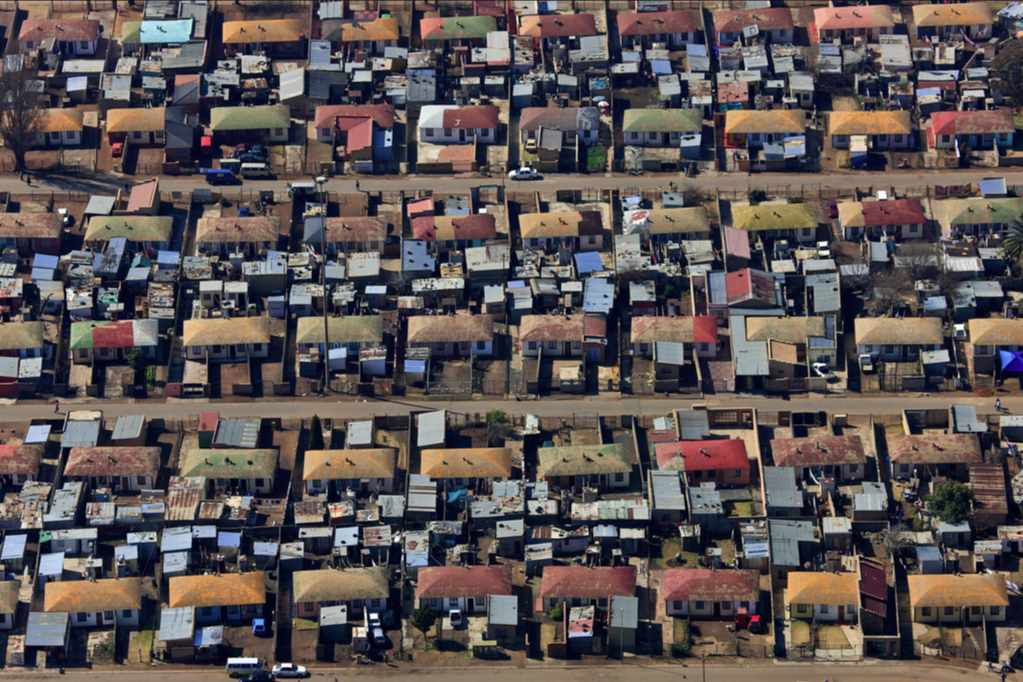
\includegraphics[scale=.25]{figures/shacks.jpg} 
 \caption{Government Housing with Backyard Shacks in Soweto}
\end{figure}

\end{frame}

%------------------------------------------------

\begin{frame}
\frametitle{This Paper}

\centering

\begin{itemize}
  \only<1>{
  \vspace{1cm}
  \item \textbf{Question}: \\ 
  \vspace{.2cm}
  {What are the urban development impacts from subsidized housing in developing contexts?}
  \vspace{.2cm}
    \begin{itemize}
      \item Evaluate household's access to services within projects and nearby.
      \vspace{1mm}
      \item Examine composition of building growth (formal and informal structures) in subsidized vs non-subsidized areas. 
      \vspace{1mm}
      \item Assess spillover effects on nearby home values in the private housing market. 
     
    \end{itemize}
  }
\vspace{.1cm}
\item<2-> \textbf{Approach:} 
\vspace{1mm}
\begin{enumerate}
      \item Leverage granular spatial data with precise geography of housing projects.
      \vspace{1mm}
      \item Use planned but unconstructed projects as additional counter-factual.
    \end{enumerate}
\vspace{.2cm}
\item<2-> \textbf{Data and Setting:} \\
\vspace{.1cm} 
{\small $\sim$ 60 public housing projects in Gauteng province combined with GPS property transactions, building-based land information, and census data.}
\end{itemize}

\end{frame}

%------------------------------------------------

\begin{frame}
\frametitle{Preview of Findings}

\centering
\begin{enumerate}


\item<1-> Significant improvement in households' access to water, sanitation, and electricity within project areas.
\vspace{2mm}
\item<2-> Public housing is direct substitute for informal housing: 

Total structure growth no different than control areas, but significant composition effects.
\vspace{2mm}
\item<3-> No evidence of amenity spillovers to neighboring areas. 

\end{enumerate}

\end{frame}

%------------------------------------------------

\section{Background}

%------------------------------------------------

\begin{frame}
\frametitle{Public Housing in South Africa}
  \begin{itemize}
    \item Large national subsidy scheme providing housing opportunities to eligible households.
    \vspace{2mm}
    \item 3 million houses delivered since program inception in 1994.\
        \begin{itemize}
          \item free-standing, single-story, two-bedrooms, 30-40$\text{m}^2$ dwellings
        \end{itemize}
    \vspace{2mm}
    \item Annual expenditure of 6bn Rands (US\$500M).
    \vspace{2mm}
    \item Supply planned by national --$>$ provincial --$>$ municipal housing agencies, project construction outsourced to private developers.
    \vspace{2mm} 
    \item Constraints on costs per unit, services access, and rooms/lot sizes.
  \end{itemize}
\end{frame}

%------------------------------------------------

\begin{frame}
\frametitle{Where are the houses built?}

\begin{itemize}
  \item Vacant private or government-owned land-plots with varying levels of (mostly informal) residential structures. 
\end{itemize}

\begin{figure}
 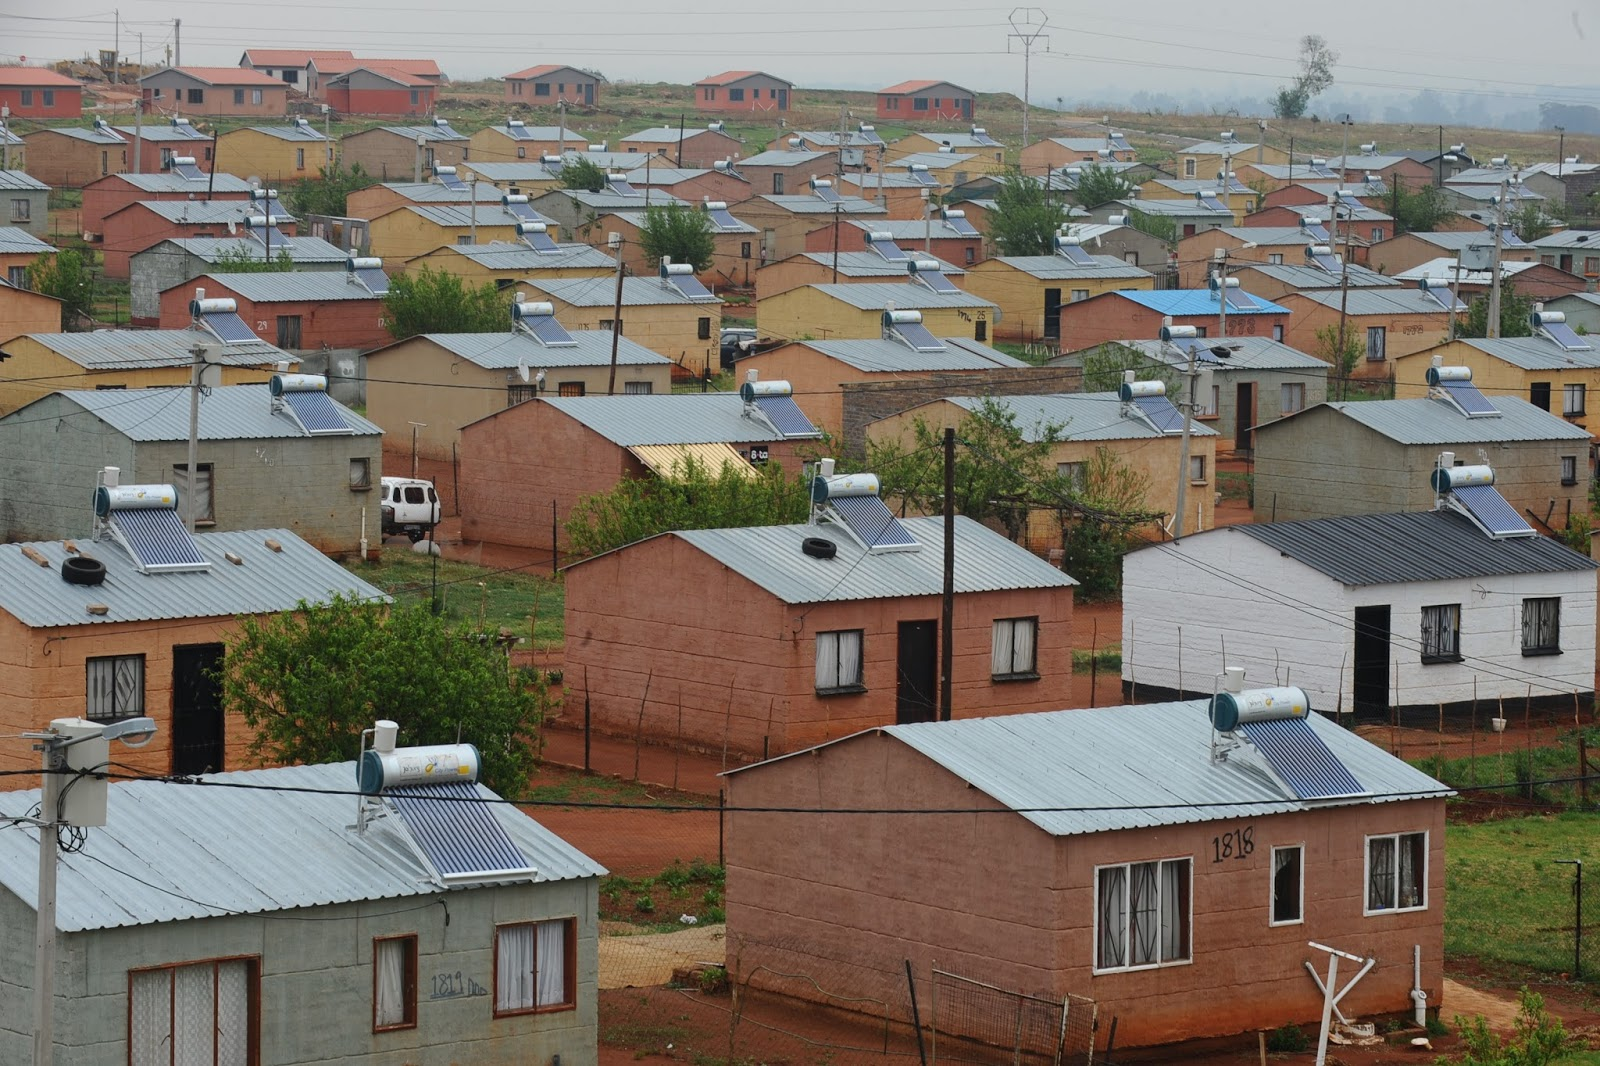
\includegraphics[scale=.125]{figures/rdp_houses.jpg} 
\end{figure}

\begin{itemize}
  \item Projects are (should be) fully serviced: roads, water, sanitation, electricity.
\end{itemize}

\end{frame}

%------------------------------------------------

        %\item Over 4.3 million houses since 1994 (13\% of pop.)
%      \item Houses 13\% of the population
%      \item Single-story, two-room (30-40$\text{m}^2$) dwellings
      %\begin{itemize}
      %  \item 50 to 500 houses per project
      %\end{itemize}
  
    %%% insert picture

%------------------------------------------------
\begin{frame}
\frametitle{Who gets a house?}
  \begin{itemize}
    \item<1-> {\bf Official Policy:}
    \vspace{2mm} 
      \begin{itemize}
        \item Must be eligible: South African Citizen, Married or with dependents, Monthly income $<$ R3,500.
        \vspace{1mm}
        \item National/provincial waiting lists.
        \vspace{1mm}
        \item No resale within 7 years.
      \end{itemize}
    \vspace{2mm}
    \item<2-> {\bf In Practice}:
      \begin{itemize}
        \vspace{2mm} 
        \item Wait-lists and eligibility weakly enforced, with many noted cases of corruption.
        \vspace{1mm}
        \item Developers often fail to meet quality requirements.
        \vspace{1mm}
        \item 20\% of houses occupied not occupied by initial owners after 5 years.
        \vspace{1mm}
        \item More than a third have backyard shacks after 2 or less years.
      \end{itemize}
  \end{itemize}

\end{frame}

%------------------------------------------------

\begin{frame}
\frametitle{Canceled/Delayed Projects}
\begin{center}

  {\footnotesize
{\it ``R95m down the tubes as housing project picked apart brick by brick''} \\ \hspace{20em}-- Timeslive, 2017 \\[.7em]
{\it ``MEC Mashatile delays Munsieville Ext 5 multimillion housing project''} \\ \hspace{20em}-- DA-GPL, 2017 \\[.7em]
{\it ``Objections put R242m housing project on hold''}\\ \hspace{20em}-- IOL News, 2016 \\[.3em]
}
\end{center}
Why?
\begin{itemize}
\item Disputes over beneficiaries; disagreement with security contractor.
\item Lack of  approval/coordination from all agencies.
\item Failed environmental impact assessment.
\end{itemize}
\end{frame}
%------------------------------------------------
%\begin{frame}
%\frametitle{Conceptual Framework: Public Housing Impacts}
%
%\begin{enumerate}
%  \item \textbf{Amenity Effect:} Upgrading housing stock/services
%    \begin{itemize}
%        \item Increase value of neighboring homes (Rossi-Hansberg [2010])
%    \end{itemize}
%\vspace{.2cm} 
%
%  \item \textbf{Crowd-In Slums:} Reduce costs of informal housing
%    \begin{itemize}
%        \item Overburden services, health/crime externalities
%        \item Reduce value of nearby houses
%    \end{itemize}
%\vspace{.2cm}
%
%  \item \textbf{Demographic Effect:} New people in the neighborhood
%    \begin{itemize}
%        \item Taste-based discrimination (Diamond and McQuade [2016])
%    \end{itemize}
%\end{enumerate}
% \end{frame}



%\begin{enumerate}
%  \item Housing externalities  {\small (Rossi-Hansberg [2010]) }
%    \begin{itemize}
%      \item Home value depends on the quality of neighboring homes
%      \item ie. informal dwellings have poor sanitation
%    \end{itemize}
%\vspace{.1cm}
%  \item Demographic externalities
%    \begin{itemize}
%      \item Taste-based discrimination
%      \item Overcrowding $\rightarrow$ crime/health externalities
%    \end{itemize}
%\vspace{.1cm}
%  \item Access to public goods (water, sewer, road infrastructure)
%\end{enumerate}


%------------------------------------------------
\section{Data and Set-up}
%------------------------------------------------


\begin{frame}
\frametitle{Data Sources}

\begin{itemize}
  \item Focus on Gauteng Province (includes Johannesburg and Pretoria)

  \vspace{2mm}

  \item<2-> Four main data sources:
  \vspace{2mm}
  \begin{enumerate}
    \item \textbf{Administrative Data on project location and planning} 
    \vspace{2mm}
    \item \textbf{Deeds-Based Housing Transactions} 
    \vspace{2mm}
    \item \textbf{Building-Based Land Use}
    \vspace{2mm}
    \item \textbf{Household Census}    
  \end{enumerate}

\end{itemize}

\end{frame}

%------------------------------------------------

\begin{frame}
\frametitle{Administrative Data on Subsidized Housing.}

  \begin{itemize}
    \item Data on location of government housing initiatives as of 2008.
    \begin{itemize} 
      \item Includes planned but unconstructed projects.
    \end{itemize}

    \item Annual Budget Reports from National Treasury. 
    
  \end{itemize}
\end{frame}

%------------------------------------------------

\begin{frame}
\frametitle{Housing Transactions}

\begin{itemize}

  \item Sourced from South African deeds registry. 
  \vspace{2mm}
  \item "Universe" of formal housing transactions recorded during 2001-2011 in
{\bf affordable areas}. (550K transactions)
  \vspace{2mm}
  \item Exact geographic location of traded property, but limited information
on characteristics other than price and lot size.
  \vspace{2mm}
  \item Includes buyer and seller name.
%\footnote{defined as census enumeration areas with mean house price value less than R500,000 in 2010.} (460K transactions) 
\end{itemize}
\end{frame}

%------------------------------------------------

\begin{frame}
\frametitle{Building Based Land-Use}

\begin{itemize}

  \item GeoTerraImage\textsuperscript{\tiny\textcopyright}: Exhaustive hand-coded building identification  from aerial imagery.
  \vspace{2mm}
  \item 2 cross-sections: 2001 and 2011. 
  \vspace{2mm}
  \item Building type differentiated by category: residential, commercial, industrial, etc.
  \vspace{2mm}
  \item Within residential, ability to differentiate formal from informal housing, including backyard shacks.
  \vspace{2mm}
  \item High Correlation ($>$80\%) with reported dwelling type from census data at coarser spatial resolution.
\end{itemize}
\end{frame}

%------------------------------------------------

\begin{frame}
\frametitle{Building Based Land-Use}

\begin{figure}
 \includegraphics[scale=.33]{figures/bblu_example.pdf} 
\end{figure}
\end{frame}

%------------------------------------------------

\begin{frame}
\frametitle{Census Data}
\begin{itemize}
  \item Full coverage from 2001 and 2011 censuses at the household level.
  \vspace{.1mm}
  \item Smallest identifiable geography is {\it\bf small area}.
  \begin{itemize}
  \item Gauteng: 11,000 small areas in 2001, 17,000 in 2011.
  \item 170 household per small area, on average.
  \end{itemize}
  \vspace{.5mm}
  \item Summary information on dwelling characteristics and access to services.
\end{itemize}
\end{frame}

%------------------------------------------------







%\begin{enumerate}
%\item \textbf{Property Transactions} measure housing projects and price impacts
%  \begin{itemize}
%    \item 500,000 deeds records (bottom 20\% of formal housing market)
%    \item Buyer/seller name, GPS, price, date from 2002-2011
%  \end{itemize}
%\vspace{.2cm}
%\item \textbf{Building Census} identifies slum-growth and in-situ upgrading
%  \begin{itemize}
%    \item 4 mil. residential buildings (50\% informal) GPS in 2001 and 2011
%  \end{itemize}
%\vspace{.2cm}
%\item \textbf{Population Census} measures demographic and economic impacts
%  \begin{itemize}
%    \item Full census for 18,000 census blocks in 2001 and 2011
%  \end{itemize}
%\vspace{.2cm}
%\item \textbf{Administrative Data} map projects (construction dates and costs)
%  \begin{itemize}
%    \item Not comprehensive
%    \item Includes planned but unconstructed projects
%  \end{itemize}




%------------------------------------------------

%  
%  
%  \item \textbf{Temporal Clustering:} include cluster with $>$50\% of transactions during modal year


\begin{frame}
\frametitle{Identifying Housing Projects}

\begin{tikzpicture}[overlay]

\onslide<1->\node[overlay,anchor=west,align=left] at (0, 2.5) {    \begin{minipage}{1\textwidth} {\begin{enumerate}
  \item \textbf{Filter on Seller Identity:} Find Governments, Housing authorities and Large Sellers from seller-names in transactions. 
\end{enumerate}}\end{minipage}};

\onslide<2->\node[overlay,anchor=west,align=left] at (0, 1.4) {    \begin{minipage}{1\textwidth} { 
\begin{enumerate}
  \setcounter{enumi}{1}
  \item \textbf{Filter on Price:} Exclude purchase prices R50,000 above yearly subsidy value for government houses.
\end{enumerate}}\end{minipage}};

\onslide<3->\node[overlay,anchor=west,align=left] at (0, .3) {    \begin{minipage}{1\textwidth} { 
\begin{enumerate}
  \setcounter{enumi}{2}
  \item \textbf{Pre-Existing Formal Dwellings:} Exclude land plots containing formal structures from 2001 building-based land-use data.
\end{enumerate}}\end{minipage}};

\onslide<4->\node[overlay,anchor=west,align=left] at (0, -.8) {    \begin{minipage}{1\textwidth} { 
\begin{enumerate}
  \setcounter{enumi}{3}
  \item \textbf{Spatial Clustering:} collect nearby houses into projects with density-based clustering algorithm. (DBSCAN)
\end{enumerate}}\end{minipage}};




\onslide<1>\node[overlay,anchor=west,align=left] at (0, -1) {
\begin{minipage}{1\textwidth} { 
\begin{figure}
\caption{Top 5 Seller Names}
\begin{tabu}{lc}
\toprule
 Seller Name & Observations \\
\midrule
City Of Johannesburg Metropolitan Municipality & 29,087  \\
City Of Johannesburg & 27,672  \\
City Of Tshwane Metropolitan Municipality & 24,780  \\
Ekurhuleni Metropolitan Municipality & 21,758  \\
Gauteng Provincial Housing Advisory Board & 13,058  \\
{\bf Total Observations }& {\bf 549,704}  \\
\bottomrule
\end{tabu}
 
\end{figure}
}\end{minipage}
} ;
% descriptive_statistics.do   program: write_biggest_sellers


\onslide<2>\node[overlay,anchor=west,align=left] at (0, -1.7) { 
\begin{minipage}{1\textwidth} { 
\begin{figure}
%\caption{Purchase Price Densities}
 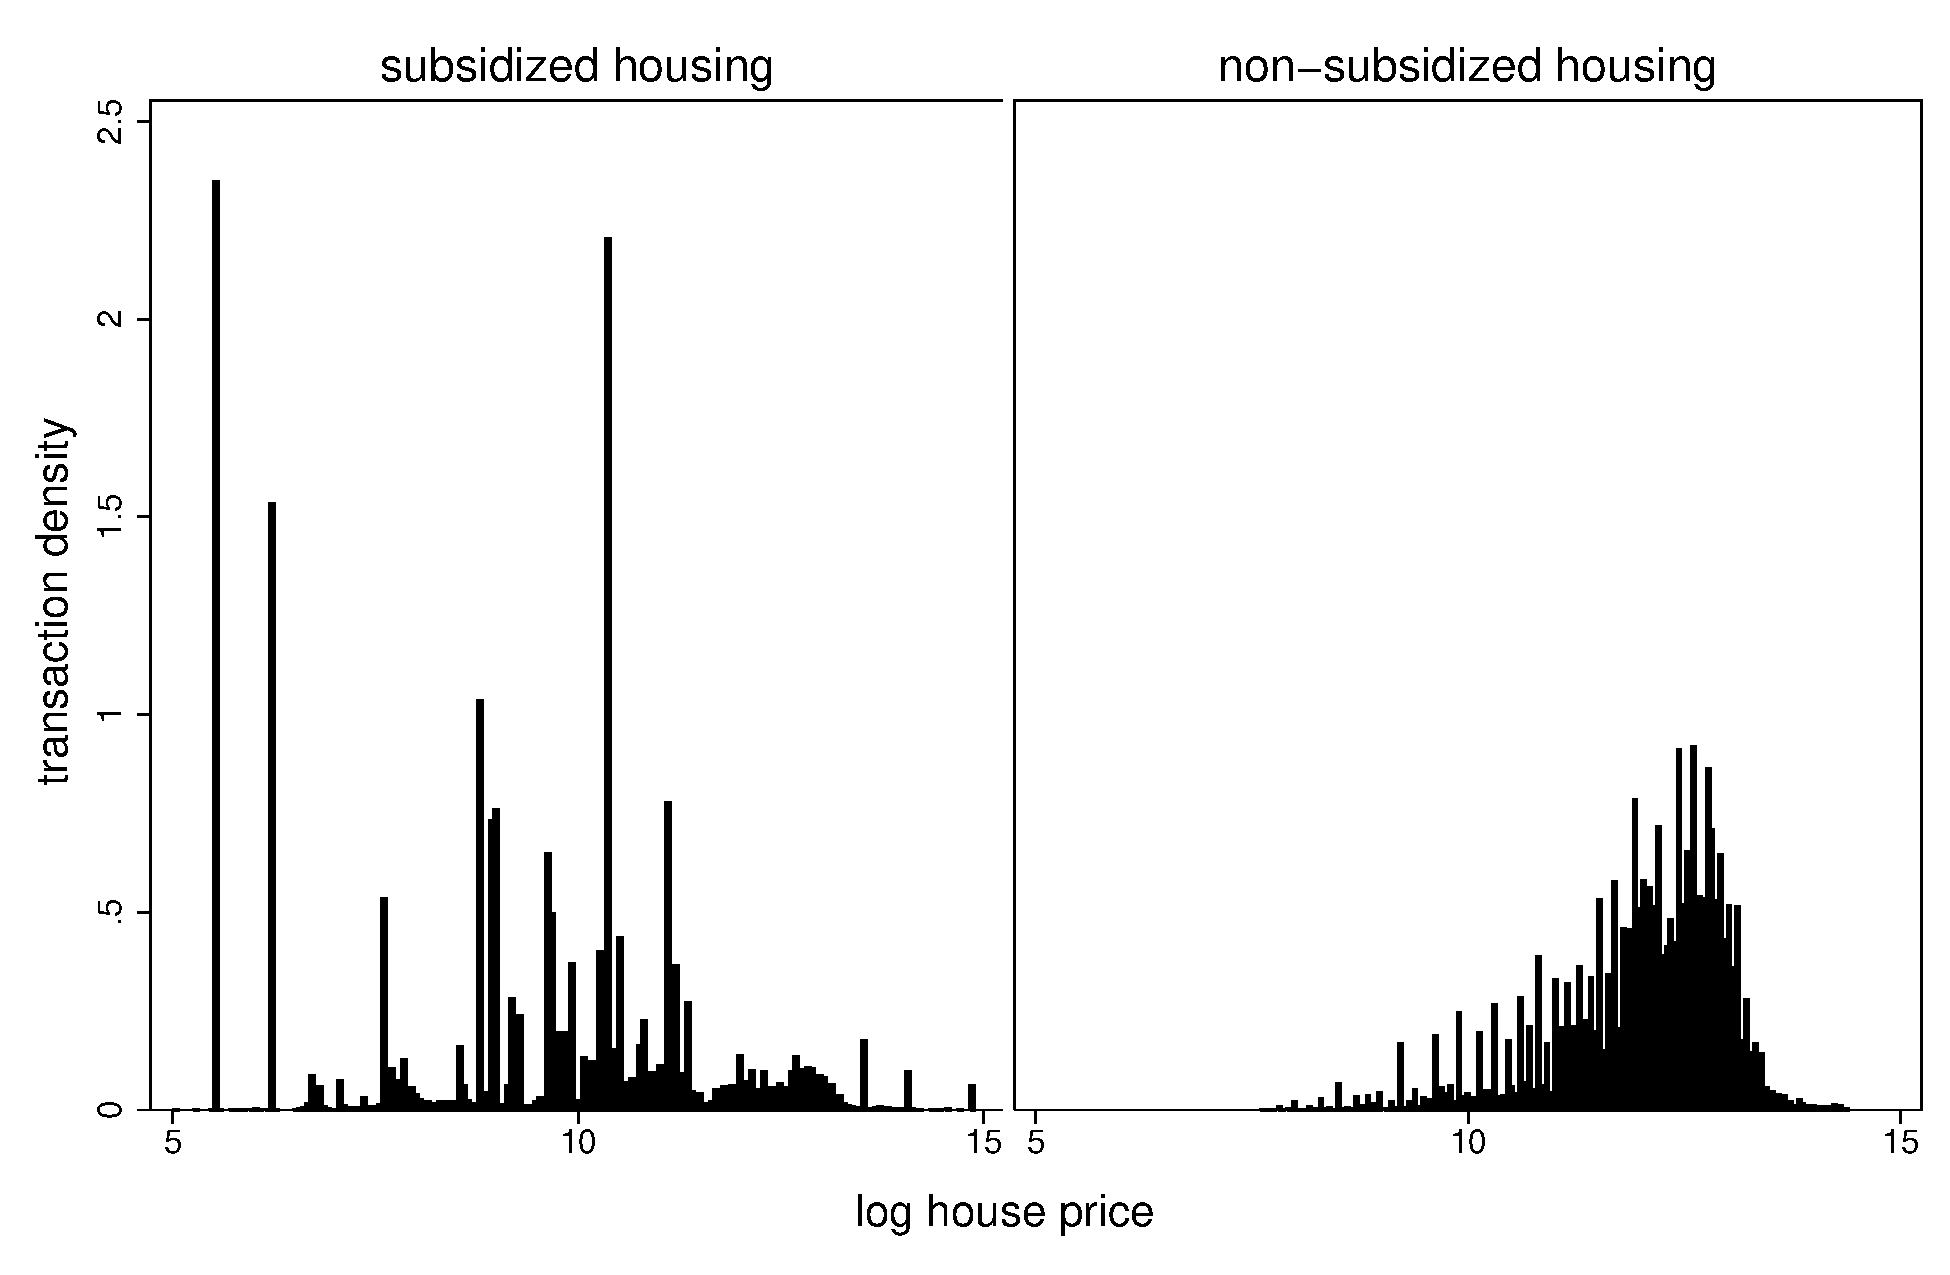
\includegraphics[scale=.23]{figures/summary_pricedist.pdf} 
\end{figure}
}\end{minipage} 
} ;
% descriptive_statistics.do   program: write_price_histogram


%\onslide<4>\node[overlay,anchor=west,align=left] at (2, -2.8) {  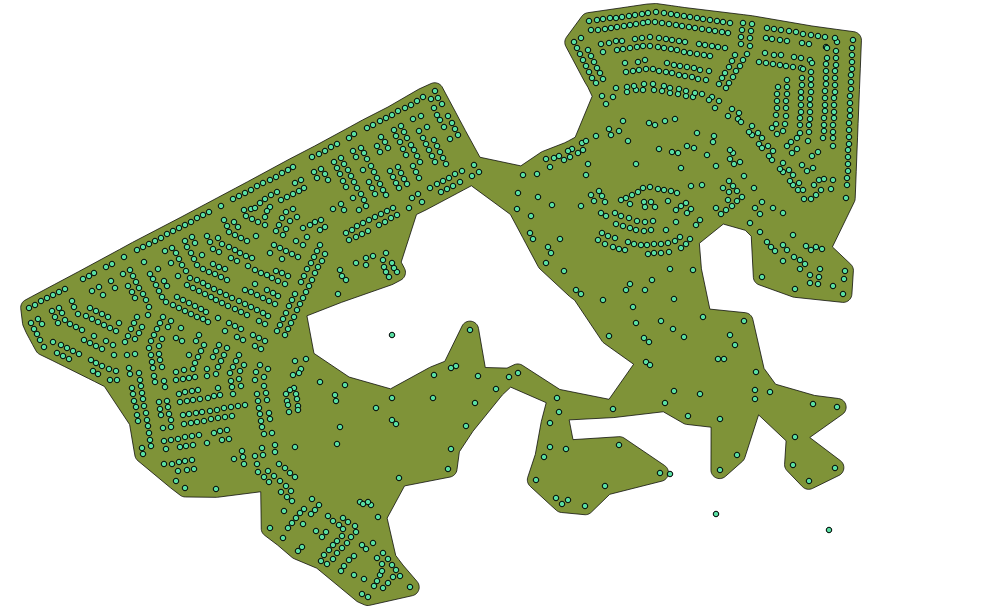
\includegraphics[scale=.16]{rdp_conhull_pic.png}  };
% generated from QGIS


\end{tikzpicture}

\end{frame}

%------------------------------------------------

\begin{frame}
\frametitle{Title}
\begin{center}
\begin{figure}
\frame{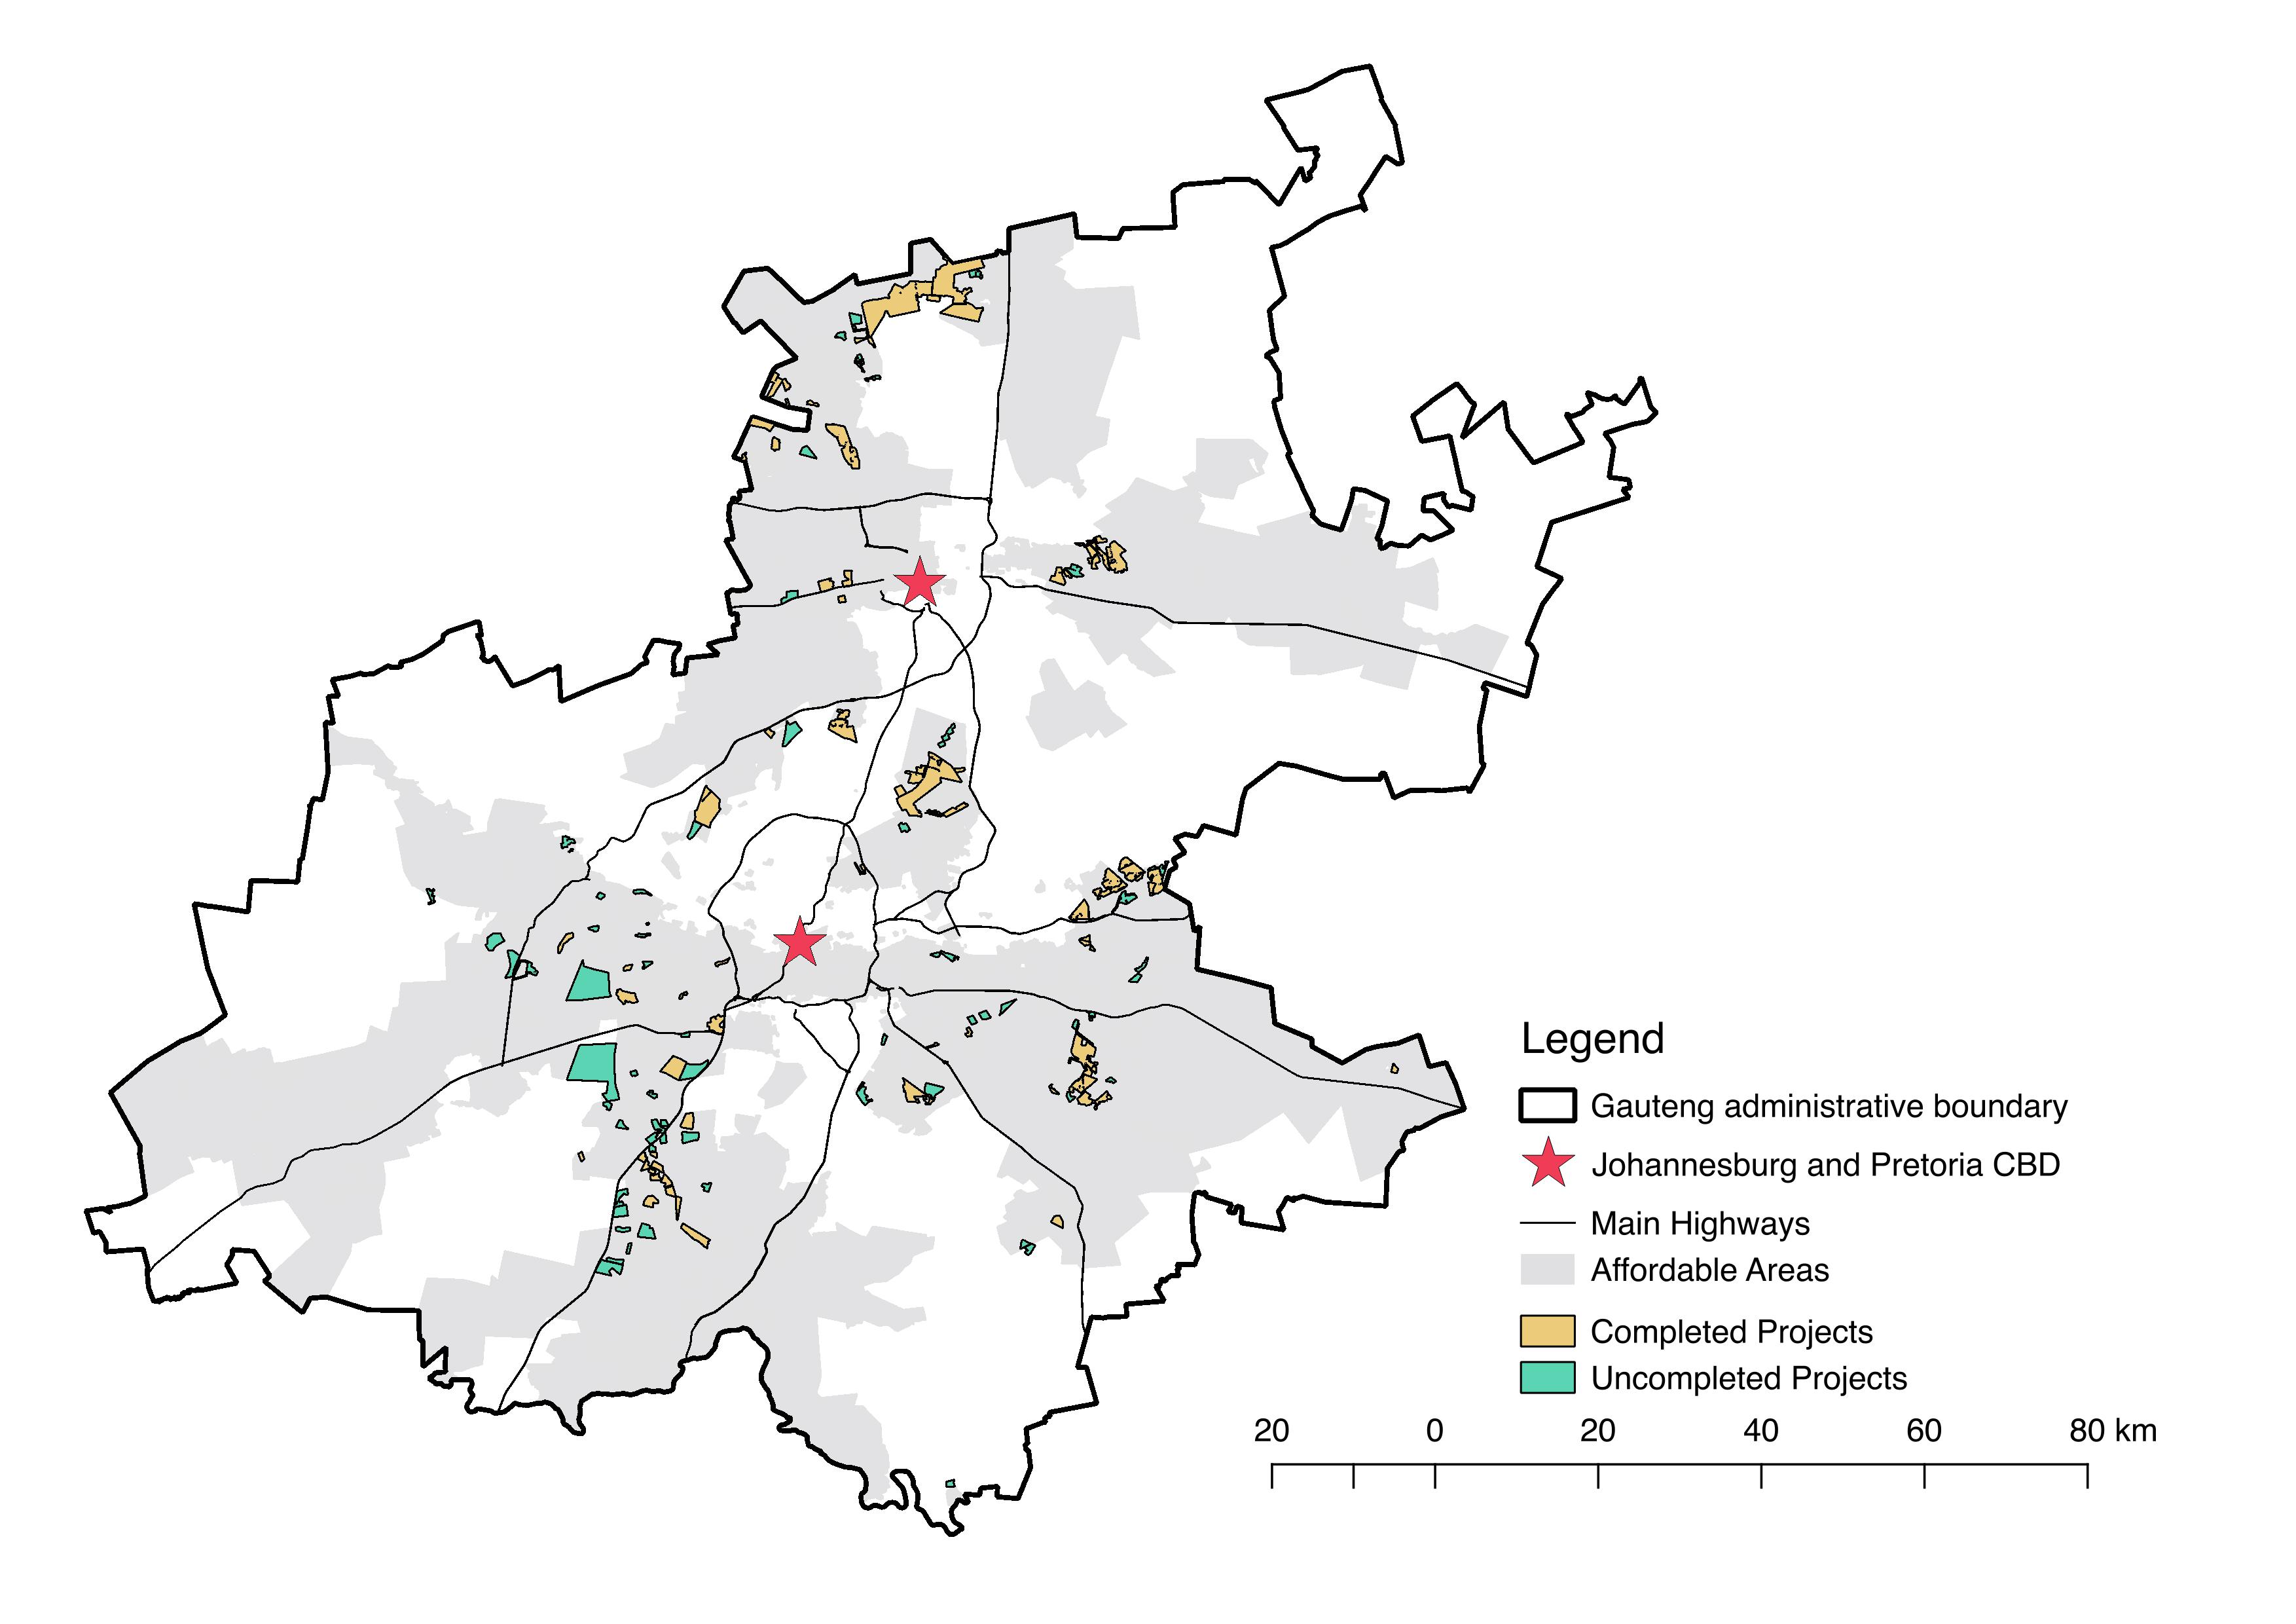
\includegraphics[scale=0.32]{datainfo/explanmap.jpg}}
\vspace{-3mm}
\end{figure}
\end{center}
\end{frame}

%------------------------------------------------


\begin{frame}
\frametitle{Identifying Planned but Unconstructed Projects}

\begin{enumerate}
  \item Admin. data have ``planned,'' ``proposed,'' ``implementing'' projects
    \begin{itemize}
      \item Exclude projects with identified project transactions
    \end{itemize}

    \vspace{.2cm}

  \item Assign projects an expected completion date
    \begin{itemize}
      \item Fuzzy-string match budget data (with start-dates) on project names
      \item Add avg. diff. between transaction-date and start-date for completed projects
    \end{itemize}
\end{enumerate}

\begin{itemize}
  \item Why are projects canceled/delayed? 
    \begin{itemize}
      \item Legal disputes, service delivery backlogs, funding complications
      \item Delays often exceed 12 years 
    \end{itemize} 
\end{itemize}

\end{frame}

%------------------------------------------------



\section{Impact on Dwelling Characteristics}

%------------------------------------------------
\begin{frame}
\frametitle{Census Areas Exposure Measures}
\only<1>{
 \begin{center}
 \begin{figure}[ht]
   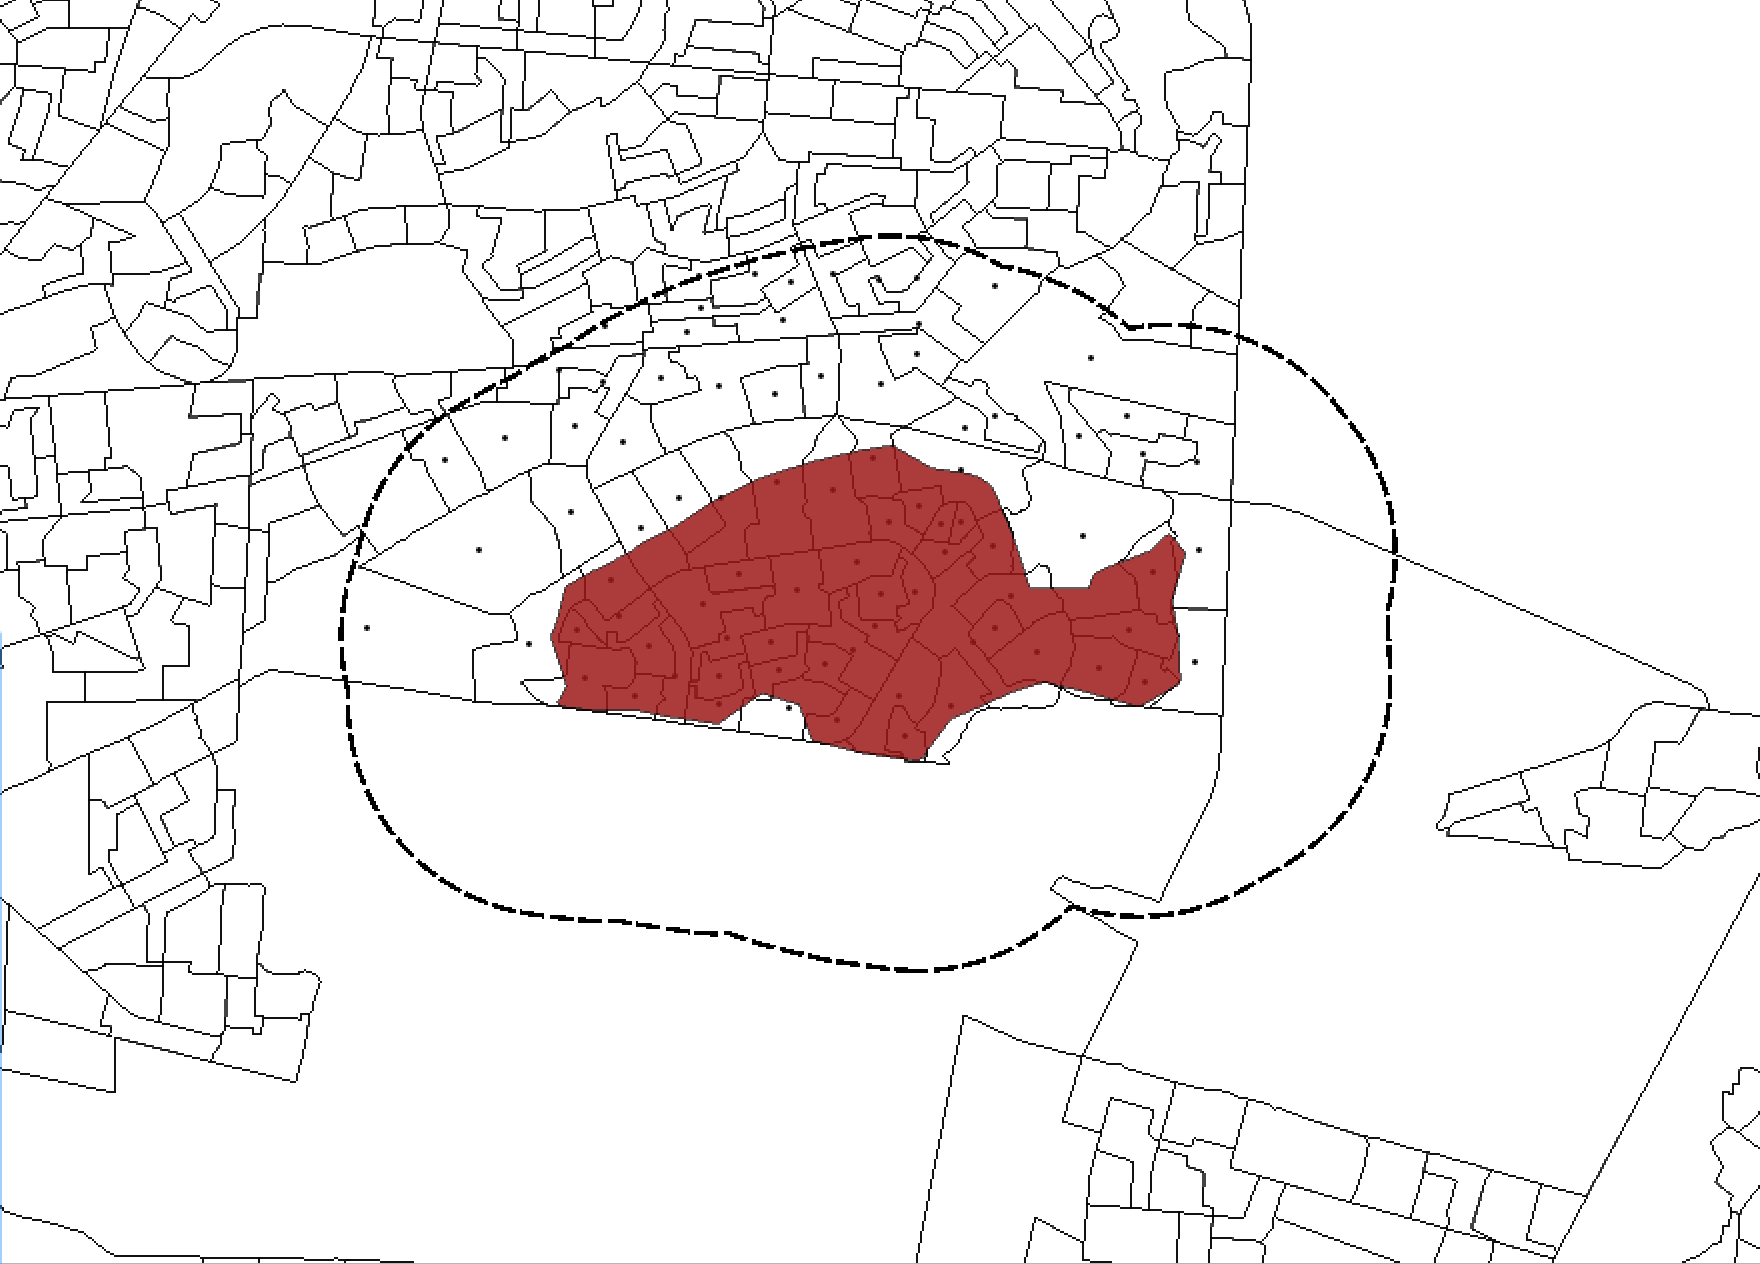
\includegraphics[scale=0.145]{design/design_5.jpg}
   \caption{\scriptsize Census "Small Areas" with centroid within 1500m of project border}
 \end{figure}
 \end{center}
}
\only<2>{
 \begin{center}
 \begin{figure}[ht]
   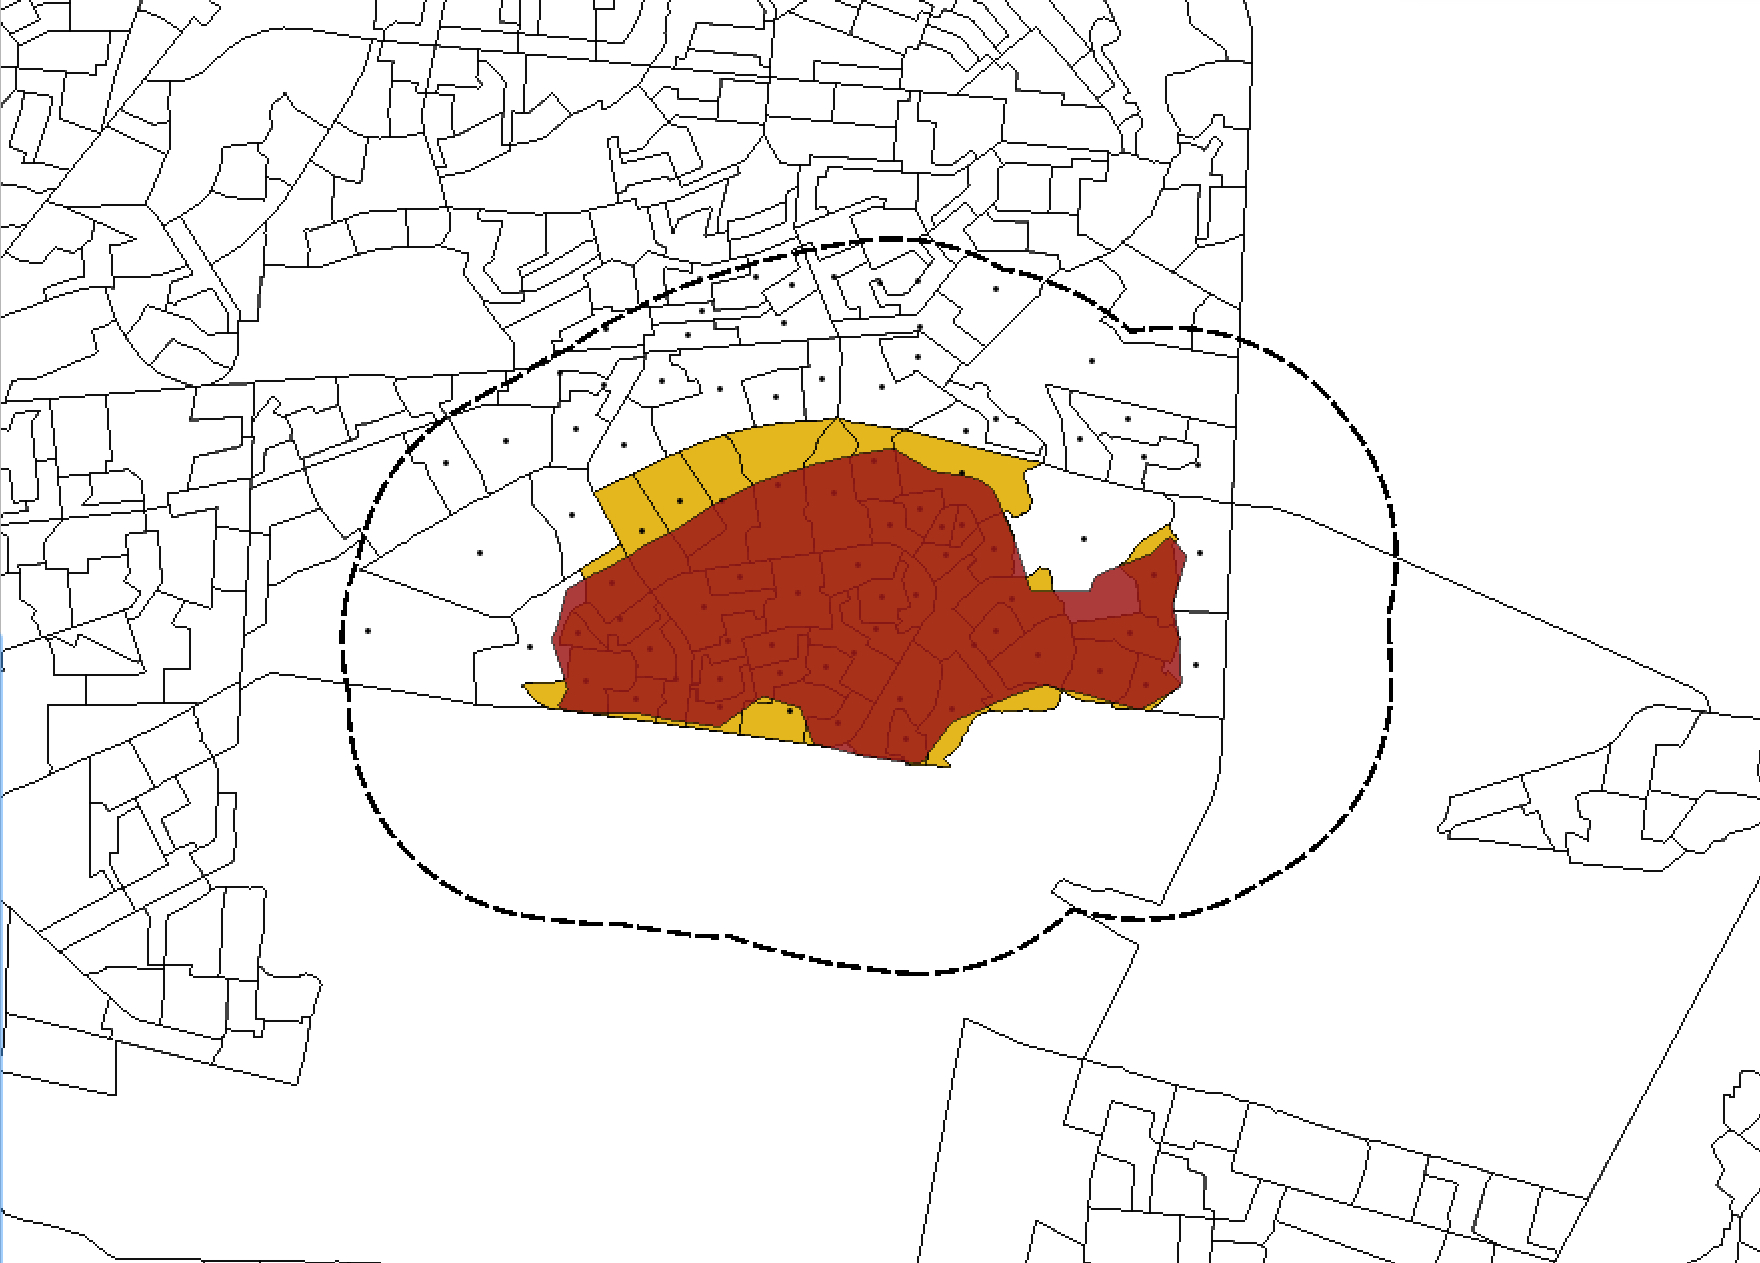
\includegraphics[scale=0.145]{design/design_6.jpg}
   \caption{\scriptsize "project" exposure: small areas with $>$ 30\% area overlap}
 \end{figure}
 \end{center}
}
\only<3>{
 \begin{center}
 \begin{figure}[ht]
   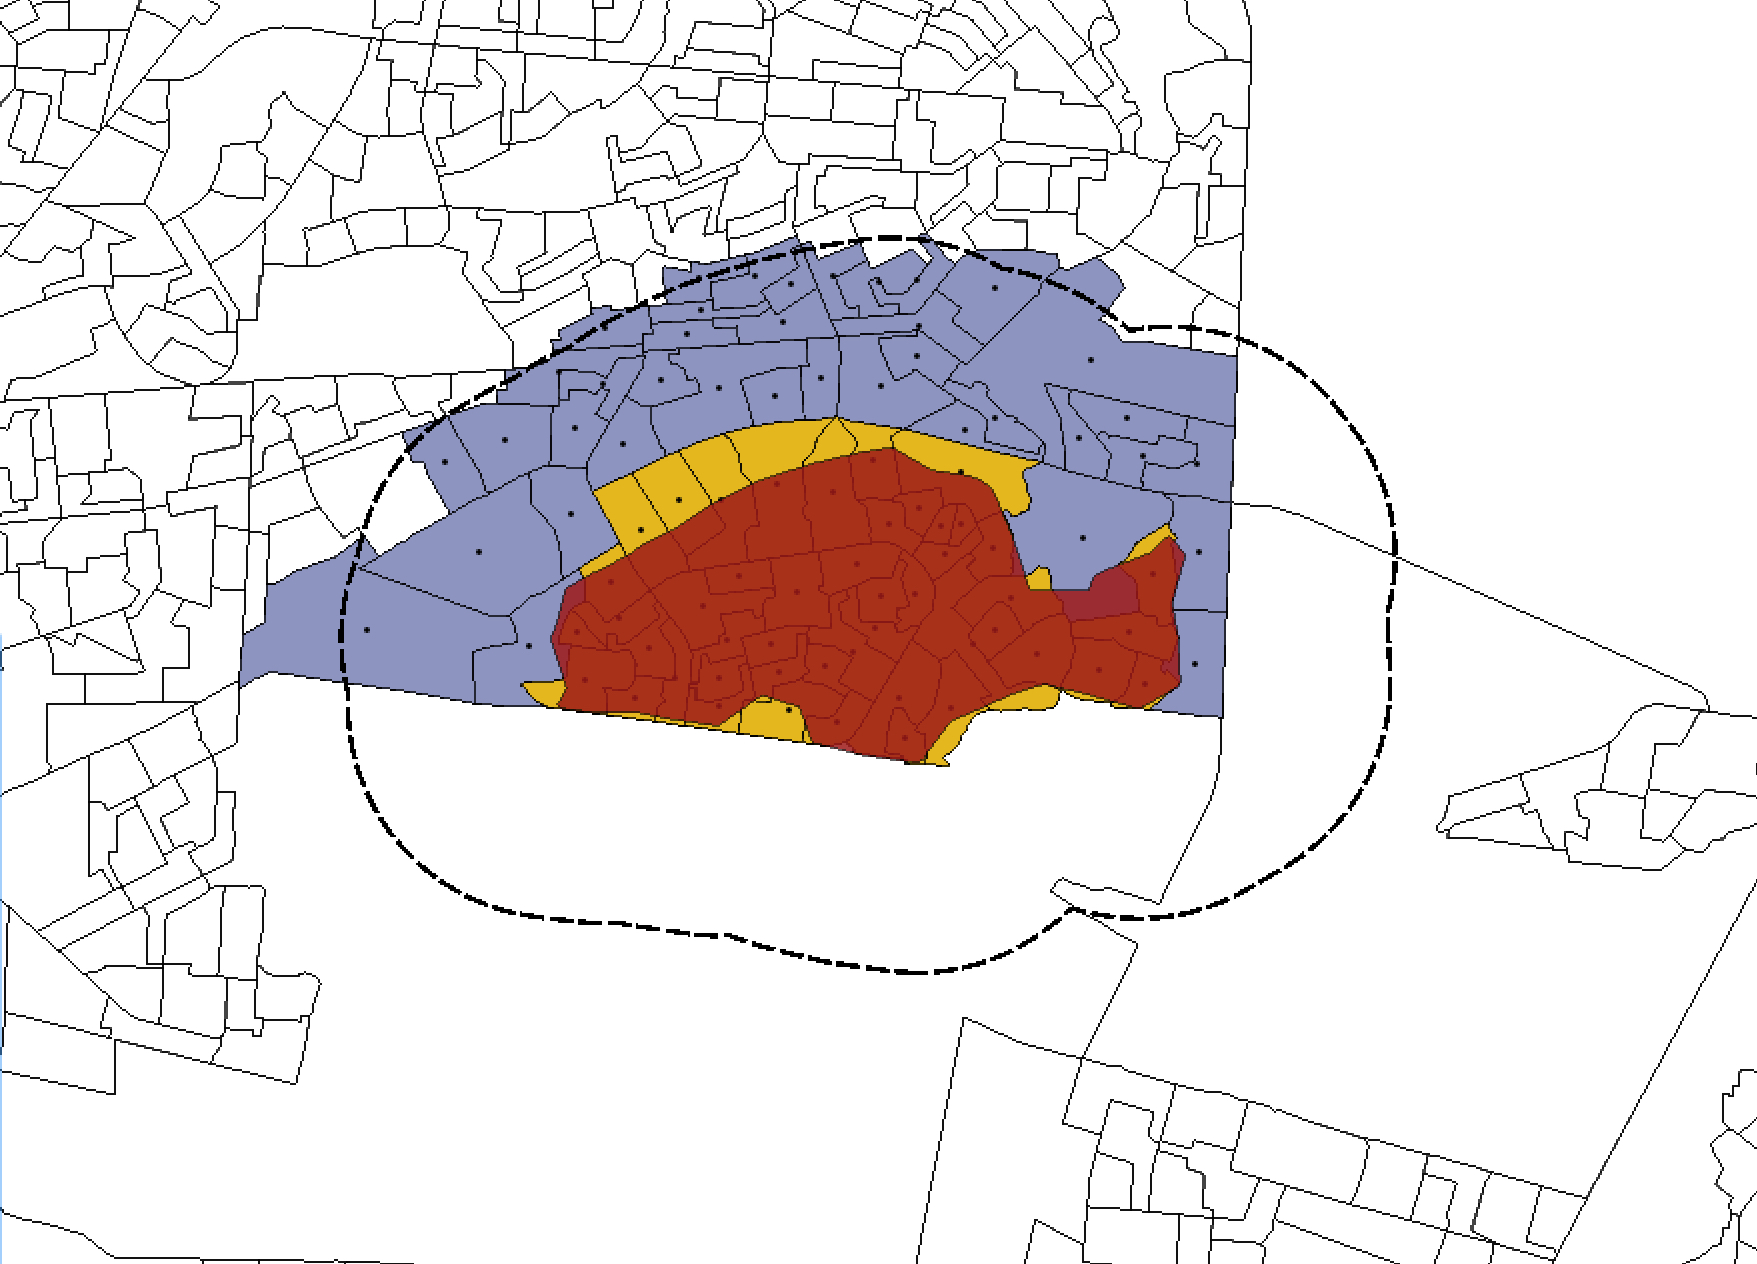
\includegraphics[scale=0.145]{design/design_7.jpg}
   \caption{\scriptsize "spillover" exposure: small areas with $<$ 30\% area overlap}
 \end{figure}
 \end{center}
}
\end{frame}


%------------------------------------------------

\begin{frame}
\frametitle{Empirical Specification}
\only<1>{
\begin{equation*}
y_{hpt} \, = \, \lambda_p + \alpha D_tC_p \, + \, \beta D_t \, + \, \gamma C_p \, + \, \varepsilon_{hpt}
\end{equation*}
}
\only<2->{
\begin{equation*}
y_{hpt} \, = \, \lambda_p + \sum\limits_{e} I^e_{hpt}\Big( \alpha^e D_tC_p \, + \, \beta^eD_t \, + \, \gamma^eC_p \, + \, \theta^e \Big) \, + \, \varepsilon_{hpt}
\end{equation*}
}
\only<1>{
with:
\begin{itemize}
\item $y_{htp}$: Outcome for household $h$ living in vicinity of project $p$, observed in census year $t$.
\item $D_{t}\,\,$=1 if year $t$ is census year 2011 (post period). 
\item $C_{p}\,\,$=1 if project $p$ has been constructed.
\item $\lambda_p$: project fixed-effect.
\item $\varepsilon_{itp}$: error term.
\end{itemize}
}
\only<2>{
with:
\begin{itemize}
\item $y_{htp}$: Outcome for household $h$ living in vicinity of project $p$, observed in census year $t$.
\item $I^e_{hpt}$=1 if household $h$ is in exposure area $e$ of project $p$.
\item $D_{t}\,\,$=1 if year $t$ is census year 2011 (post period). 
\item $C_{p}\,\,$=1 if project $p$ has been constructed.
\item $\lambda_p$: project fixed-effect.
\item $\varepsilon_{itp}$: error term.
\end{itemize}
}
\only<3>{
\begin{itemize}
\item $\alpha^e$ is the DD effect of housing projects on outcome $y$ at exposure $e$, comparing constructed vs. non-constructed projects, before and after construction.
\item Assumes no differential trends between treatment and control areas, absent of project construction.
\item concerns:
\begin{itemize}
  \item correlation between what stopped project.
  \item endogenous census geography.
  \item "dosage".
\end{itemize}
\end{itemize}
}
\only<4>{
{\bf Outcomes:}
\begin{itemize}
\item water and sewers: whether households have a flush toilets, access to an indoors water tap, water from utility company. 
\item main energy sources for cooking, heating and lighting.
\item whether household live in a formal house and whether they own it.
\item population and household density.
\end{itemize}
}
\end{frame}


%------------------------------------------------

\begin{frame}
\only<1>{
\frametitle{Effect On Dwelling Characteristics I. (Nearby Projects)}
\vspace{-1.5mm}
\begin{table}
{\footnotesize
{\footnotesize
\definecolor{o}{RGB}{237,189,100}  
\def\sym#1{\ifmmode^{#1}\else\(^{#1}\)\fi}
\begin{tabular}{l*{5}{c}}
          &\multicolumn{1}{c}{flush toilet}         &\multicolumn{1}{c}{water tap}         &\multicolumn{1}{c}{utility water}         &\multicolumn{1}{c}{owner}         &\multicolumn{1}{c}{house}         \\[0.2em]
\hline\\[-0.9em]
%------------------------------------------------------------------------------------------------
\rowcolor{o} spillover\_DD  &  0.017    &   -0.011     &   -0.005    &   -0.019    &   -0.012   \\
\rowcolor{o}                & (0.037)   &  (0.033)     &  (0.013)    &  (0.029)    &  (0.030)         \\
[.5em]
spillover\_post& 0.069\sym{**} &  0.177\sym{***}&  0.006    &   -0.030\sym{*}  &    0.077\sym{***}\\
               &  (0.027)      &  (0.024)       &  (0.010)  &  (0.017)         &  (0.023)  \\       
[.5em]
spillover\_complete & -0.016   &    0.004       &    0.013  &    0.029         &    0.067      \\
                    & (0.052)  &  (0.049)       &  (0.017)  &  (0.032)         &  (0.043)         \\
[.5em]
spillover &  -0.023    &   -0.041    &   -0.003    &   -0.008    &   -0.029         \\
          &  (0.039)   &  (0.038)    &  (0.014)    &  (0.023)    &  (0.033)         \\
%------------------------------------------------------------------------------------------------
[.3em]
& \multicolumn{5}{c}{...}\\
[.5em]
\hline \\[-0.9em]
$\bar{y}$ 2001& 0.747      &    0.345        &    0.948      &    0.511         &    0.550         \\
$\bar{y}$ 2011& 0.822      &    0.518        &    0.936      &    0.457         &    0.623         \\
N          &  3,214,472    &  3,214,472      &  3,214,472    &  3,112,425       &  3,067,560       \\
R$^{2}$    &    0.231      &    0.147        &    0.062      &    0.064         &    0.110         \\
\hline
\multicolumn{6}{l}{\tiny All specifications include project Fixed Effects. Standard errors clustered at the project level.}
\end{tabular}
}

}
\end{table}
}
\only<2>{
\frametitle{Effect On Dwelling Characteristics I. (Inside Projects)}
\vspace{-1.5mm}
\begin{table}
{\footnotesize
{\footnotesize
\definecolor{o}{RGB}{237,189,100}  
\def\sym#1{\ifmmode^{#1}\else\(^{#1}\)\fi}
\begin{tabular}{l*{5}{c}}
          &\multicolumn{1}{c}{flush toilet}         &\multicolumn{1}{c}{water tap}         &\multicolumn{1}{c}{utility water}         &\multicolumn{1}{c}{owner}         &\multicolumn{1}{c}{house}         \\[0.2em]
\hline\\[-0.9em]
& \multicolumn{5}{c}{...}\\
[.5em]
%------------------------------------------------------------------------------------------------
\rowcolor{o} project\_DD  &  0.137\sym{**} &  0.143\sym{***}&   0.036       &   -0.085         &    0.158\sym{***}\\
\rowcolor{o} &  (0.065)       &  (0.052)       &  (0.038)      &  (0.073)         &  (0.055)         \\
[.5em]
project\_post&    0.068     &   0.087\sym{**} &   -0.028      &    0.036         &    0.065\sym{*}  \\
            &  (0.048)     &  (0.040)        &  (0.036)      &  (0.039)         &  (0.036)         \\
[.5em]
project\_completed& 0.100   &    0.030        &    0.036      &    0.124         &    0.105         \\
                 &(0.120)  &  (0.082)        &  (0.033)      &  (0.081)         &  (0.092)         \\
[.5em]
project    &-0.343\sym{***}& -0.251\sym{***} &  -0.038       & -0.187\sym{***}  &   -0.263\sym{***}\\
           &  (0.089)      &  (0.059)        &  (0.028)      &  (0.056)         &  (0.076)         \\
%------------------------------------------------------------------------------------------------
          \\[-0.9em]
\hline \\[-0.9em] 
$\bar{y}$ 2001& 0.747      &    0.345        &    0.948      &    0.511         &    0.550         \\
$\bar{y}$ 2011& 0.822      &    0.518        &    0.936      &    0.457         &    0.623         \\
N          &  3,214,472    &  3,214,472      &  3,214,472    &  3,112,425       &  3,067,560       \\
R$^{2}$    &    0.231      &    0.147        &    0.062      &    0.064         &    0.110         \\
\hline
\multicolumn{6}{l}{\tiny All specifications include project Fixed Effects. Standard errors clustered at the project level.}
\end{tabular}
}

}
\end{table}
}
\end{frame}

%------------------------------------------------

\begin{frame}
\only<1>{
\frametitle{Effect On Dwelling Characteristics II. (Nearby Projects)}
\vspace{-1.5mm}
\begin{table}
{\footnotesize
{\footnotesize
\definecolor{o}{RGB}{237,189,100}  
\def\sym#1{\ifmmode^{#1}\else\(^{#1}\)\fi}
\begin{tabular}{l*{5}{c}}
          &\multicolumn{1}{c}{elec cooking} &\multicolumn{1}{c}{elec heat}  &\multicolumn{1}{c}{elec light}         &\multicolumn{1}{c}{hh density}         &\multicolumn{1}{c}{pop density}      \\[0.2em]
\hline\\[-0.9em]
%------------------------------------------------------------------------------------------------
\rowcolor{o} spillover\_DD  & -0.004   &   -0.065  &   -0.053   &  345.6\sym{*}  &  579.8     \\
\rowcolor{o}                &  (0.039) &  (0.047)  &  (0.037)   &(205.3)         &(445.8)     \\ 
[.5em]
spillover\_post & 0.170\sym{***}&0.131\sym{***} &0.118\sym{***} & 270.2\sym{**} &  625.1\sym{**} \\
                & (0.031)       &  (0.027)      &  (0.033)      &(118.8)        &(278.1)       \\       
[.5em]
spillover\_complete &  -0.017    &    0.005    &    0.019     & -118.7      &  -69.4        \\
                    &  (0.042)   &  (0.044)    &  (0.043)     &(302.5)      &(753.3)        \\
[.5em]
spillover &   -0.044    &   -0.036   &   -0.033    &  284.4   &  654.5         \\
          &  (0.035)    &  (0.033)   &  (0.036)    &(204.1)   &(505.2)         \\
%------------------------------------------------------------------------------------------------
[.3em]
& \multicolumn{5}{c}{...}\\
[.5em]
\hline \\[-0.9em]
$\bar{y}$ 2001& 0.644      &    0.617       &    0.751       &2,167.9      &7,192.7         \\
$\bar{y}$ 2011& 0.821      &    0.716       &    0.842       &2,869.2      &8,354.4         \\
N          &  3,214,472    &  3,214,472     &  3,214,472     & 15,454        &    15,454         \\
R$^{2}$    & 0.193         &    0.152       &    0.168       &    0.301      &    0.303         \\
\hline
\multicolumn{6}{l}{\tiny All specifications include project Fixed Effects. Standard errors clustered at the project level.}
\end{tabular}
}

}
\end{table}
}
\only<2>{
\frametitle{Effect On Dwelling Characteristics II. (Inside Projects)}
\vspace{-1.5mm}
\begin{table}
{\footnotesize
{\footnotesize
\definecolor{o}{RGB}{237,189,100}  
\def\sym#1{\ifmmode^{#1}\else\(^{#1}\)\fi}
\begin{tabular}{l*{5}{c}}
          &\multicolumn{1}{c}{elec cooking} &\multicolumn{1}{c}{elec heat}  &\multicolumn{1}{c}{elec light}         &\multicolumn{1}{c}{hh density}         &\multicolumn{1}{c}{pop density}    
          \\[0.2em]
\hline\\[-0.9em]
& \multicolumn{5}{c}{...}\\
[.5em]
%------------------------------------------------------------------------------------------------
\rowcolor{o} project\_DD &  0.294\sym{***} &  0.209\sym{***} &  0.116   & -127.3  & -328.5     \\
\rowcolor{o}             &  (0.070)        &  (0.067)        &  (0.081) &(864.7)  &(1,631.7)\\
[.5em]
project\_post & 0.168\sym{***}& 0.142\sym{**} & 0.143\sym{**} &1,265.5\sym{*} &2,635.3\sym{*}  \\
              &  (0.060)       &  (0.056)      &  (0.066)      &(714.9)        &(1,376.0)       \\
[.5em]
project\_completed & -0.038    &   -0.022      &    0.111      & -928.7\sym{*} &-1,384.9  \\
                   & (0.099)   &  (0.088)      &  (0.110)      & (495.1)       &(1,254.1) \\
[.5em]
project     & -0.359\sym{***} & -0.329\sym{***}&-0.369\sym{***}&  835.1\sym{**}&1,649.6         \\
            &  (0.071)        &  (0.068)       &  (0.081)      &(383.7)        &(1,005.9)       \\
%------------------------------------------------------------------------------------------------
          \\[-0.9em]
\hline \\[-0.9em] 
$\bar{y}$ 2001& 0.644      &    0.617       &    0.751       &2,167.9      &7,192.7         \\
$\bar{y}$ 2011& 0.821      &    0.716       &    0.842       &2,869.2      &8,354.4         \\
N          &  3,214,472    &  3,214,472     &  3,214,472     & 15,454        &    15,454         \\
R$^{2}$    & 0.193         &    0.152       &    0.168       &    0.301      &    0.303         \\
\hline
\multicolumn{6}{l}{\tiny All specifications include project Fixed Effects. Standard errors clustered at the project level.}
\end{tabular}
}

}
\end{table}
}
\end{frame}

%------------------------------------------------

\section{Impact on Building Density}

%------------------------------------------------

\begin{frame}
\frametitle{Gridded Building Density Measure}
\only<1>{
 \begin{center}
 \begin{figure}[ht]
   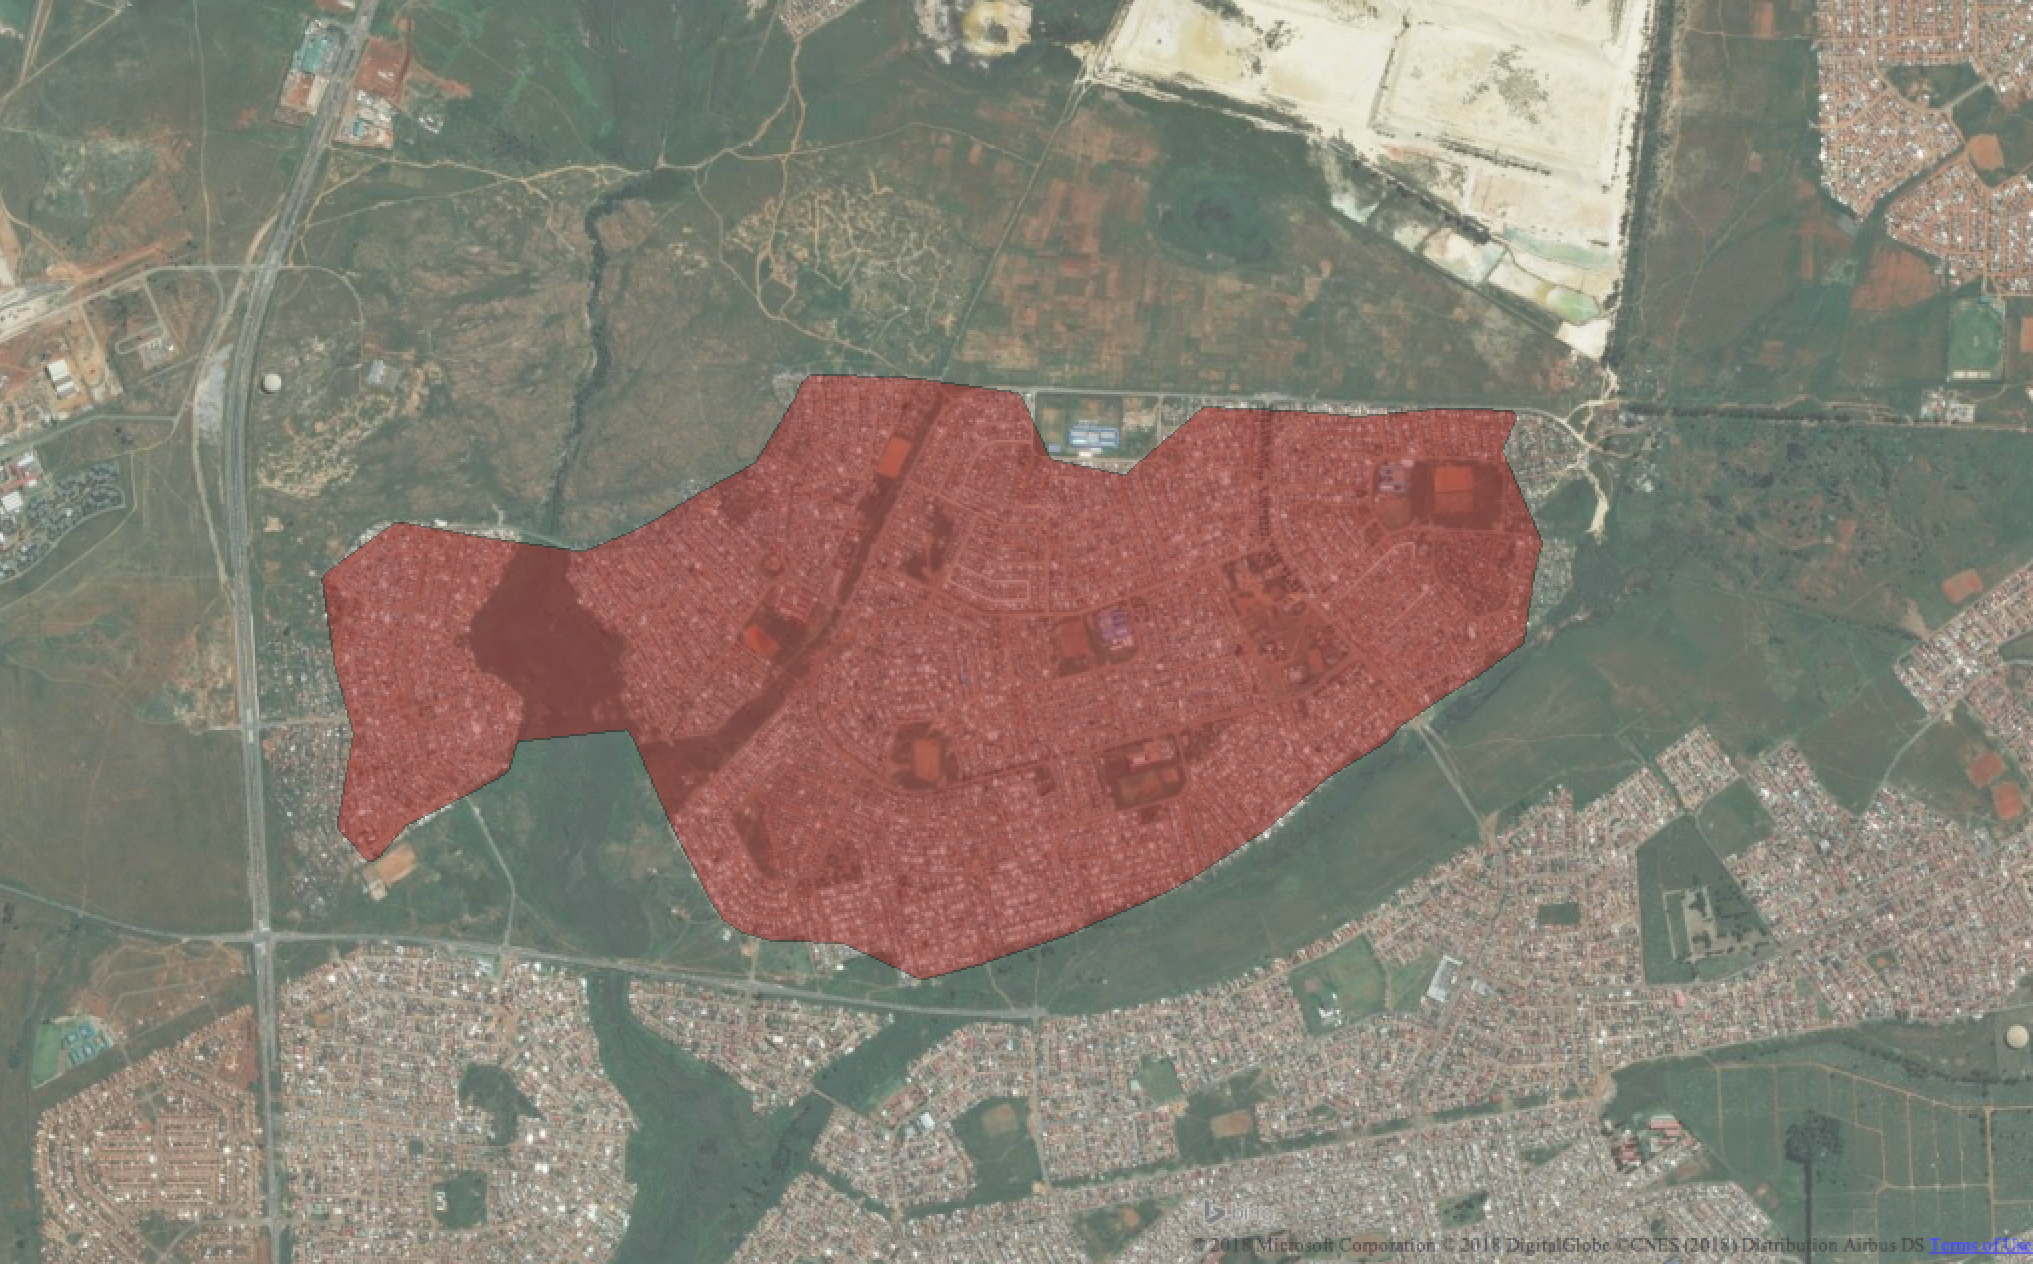
\includegraphics[scale=0.27]{design/bbludesign1.png}
   \caption{\scriptsize Empirical design for building density regressions}
 \end{figure}
 \end{center}
}
\only<2>{
 \begin{center}
 \begin{figure}[ht]
   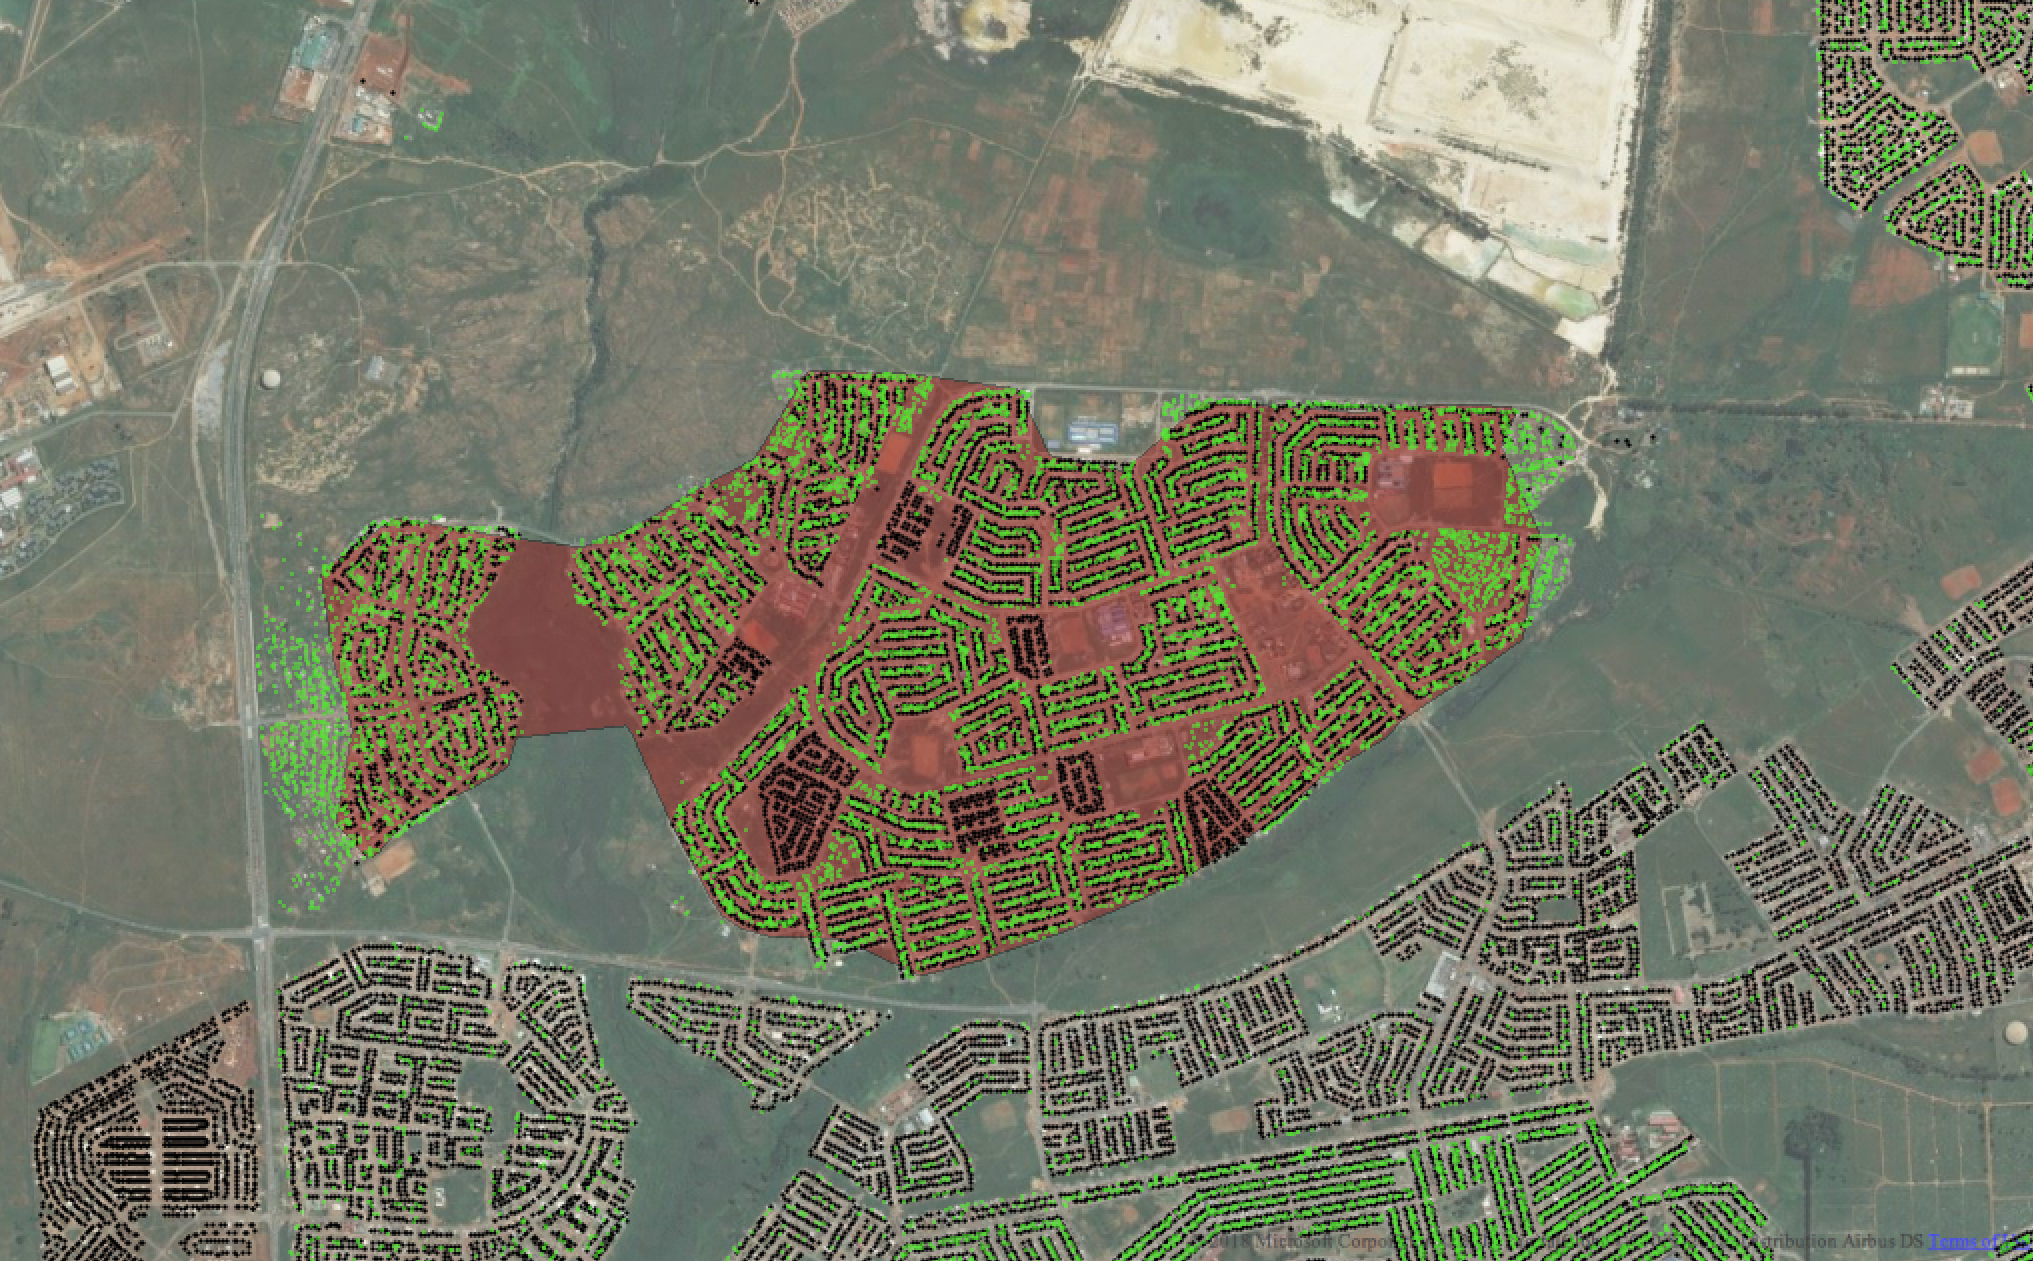
\includegraphics[scale=0.27]{design/bbludesign2.png}
   \caption{\scriptsize BBLU data showing formal (black) and informal (green) residential structures}
 \end{figure}
 \end{center}
}
\only<3>{
 \begin{center}
 \begin{figure}[ht]
   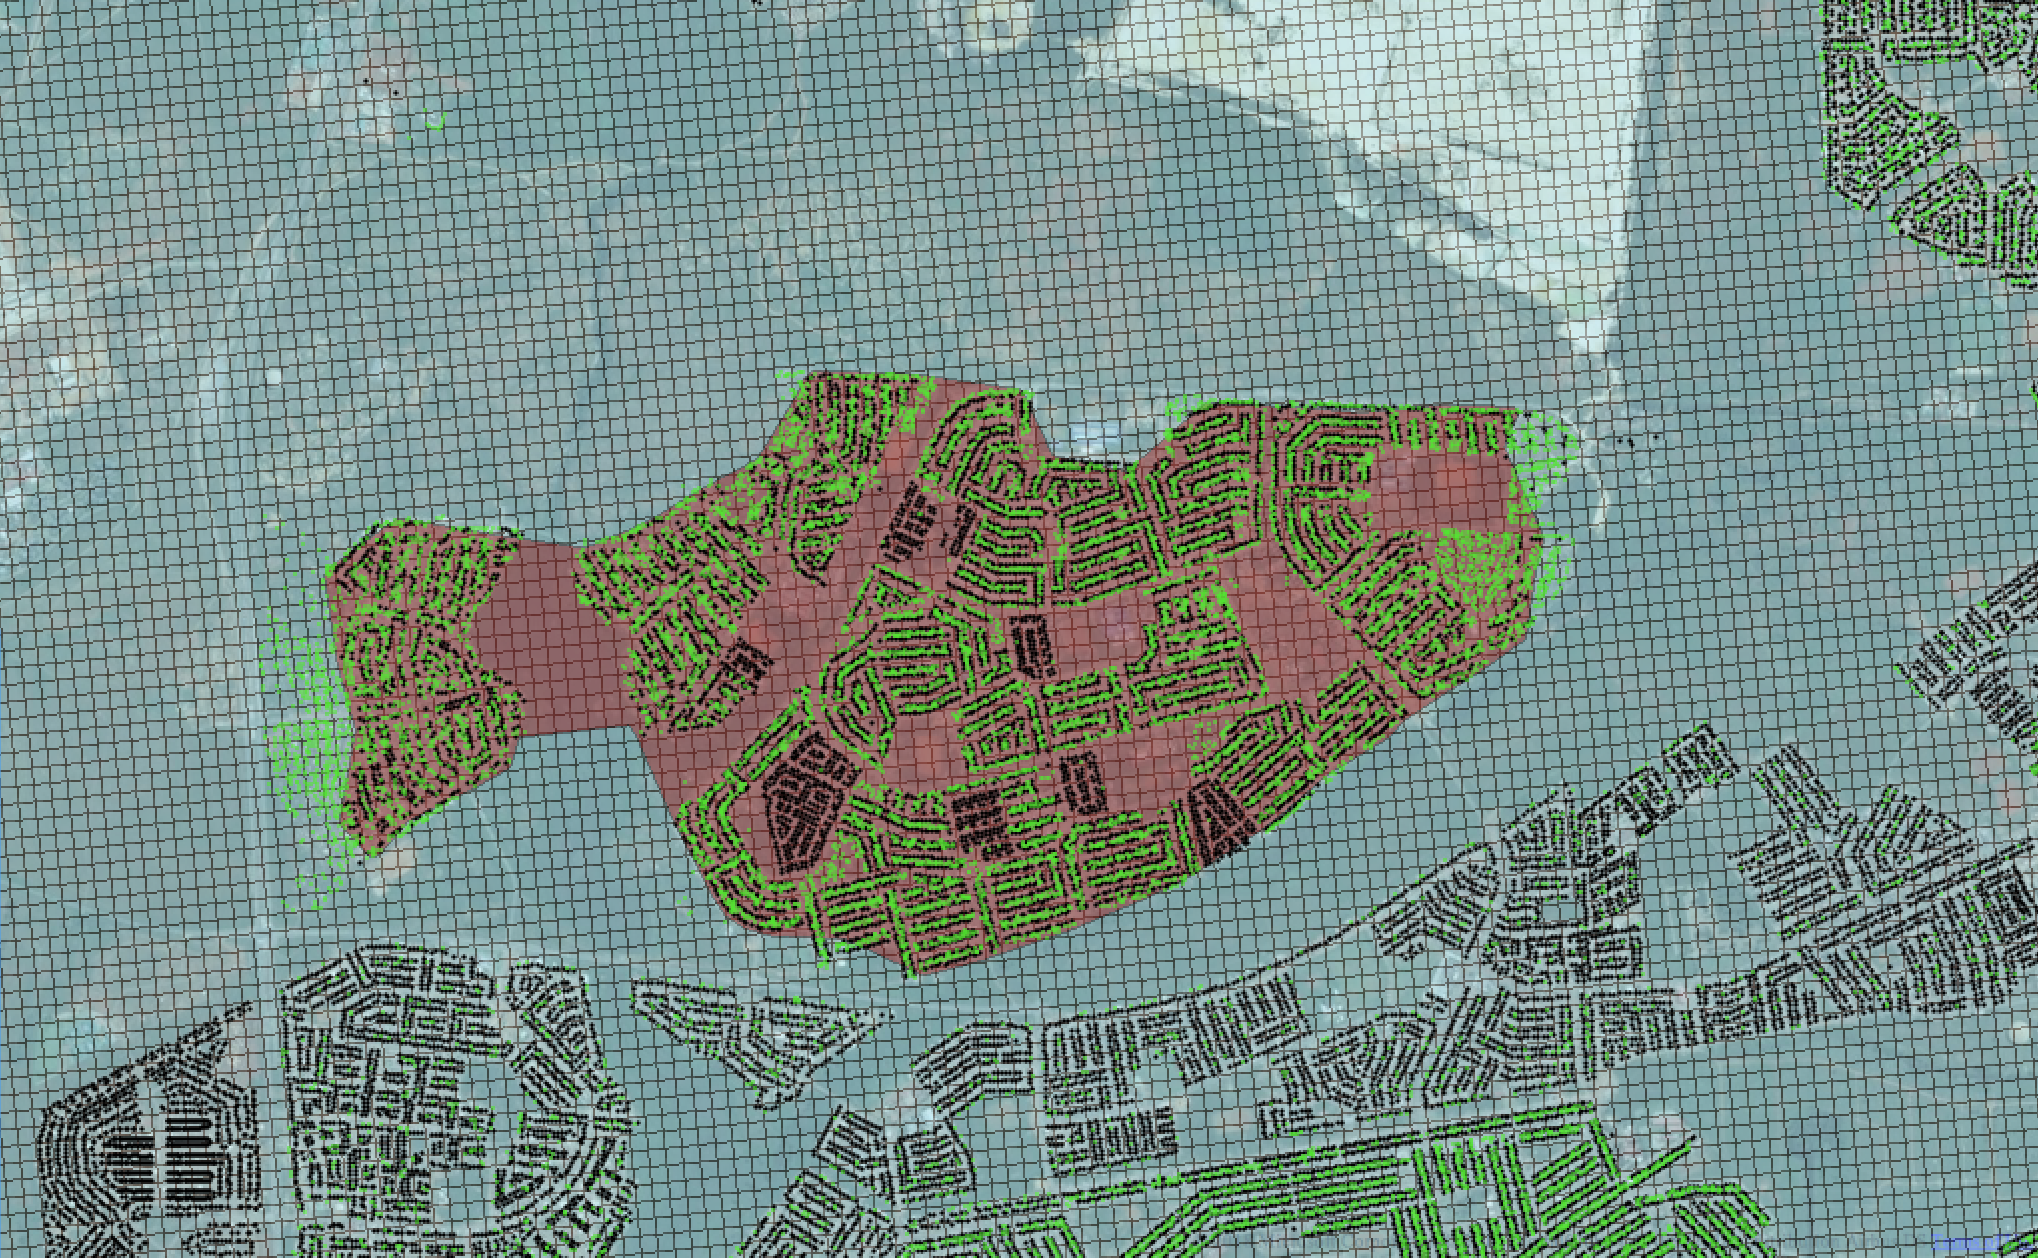
\includegraphics[scale=0.27]{design/bbludesign3.png}
   \caption{\scriptsize 50m $\times$ 50m grid overlay.}
 \end{figure}
 \end{center}
}
\only<4>{
 \begin{center}
 \begin{figure}[ht]
   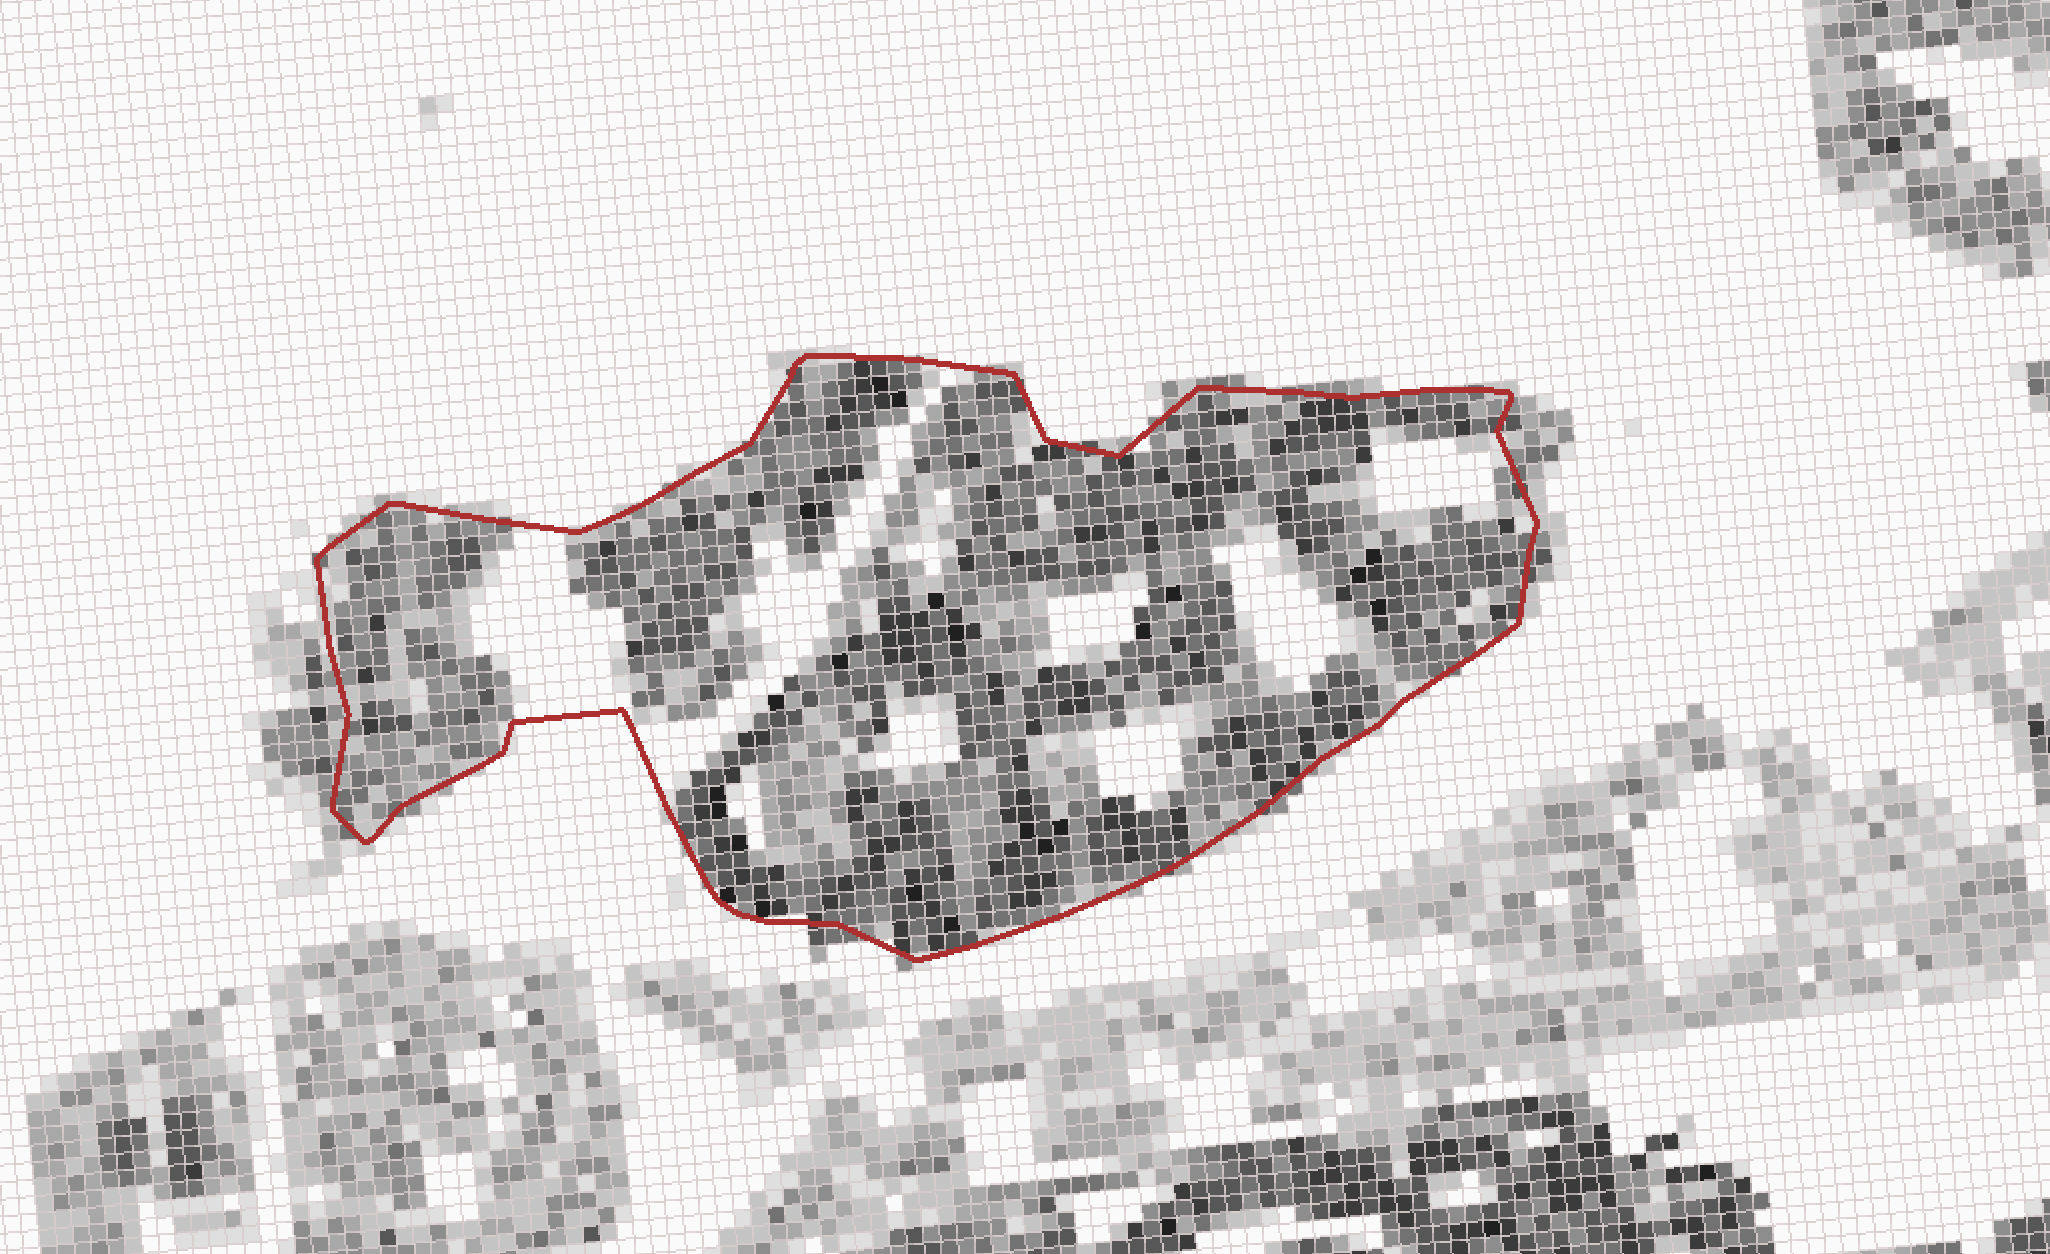
\includegraphics[scale=0.27]{design/bbludesign4.png}
   \caption{\scriptsize Aggregated data at the cell level.}
 \end{figure}
 \end{center}
}
\end{frame}

%------------------------------------------------

\begin{frame}
\frametitle{Raw Density Means }
\only<1>{
 \begin{center}
 \begin{figure}[ht]
   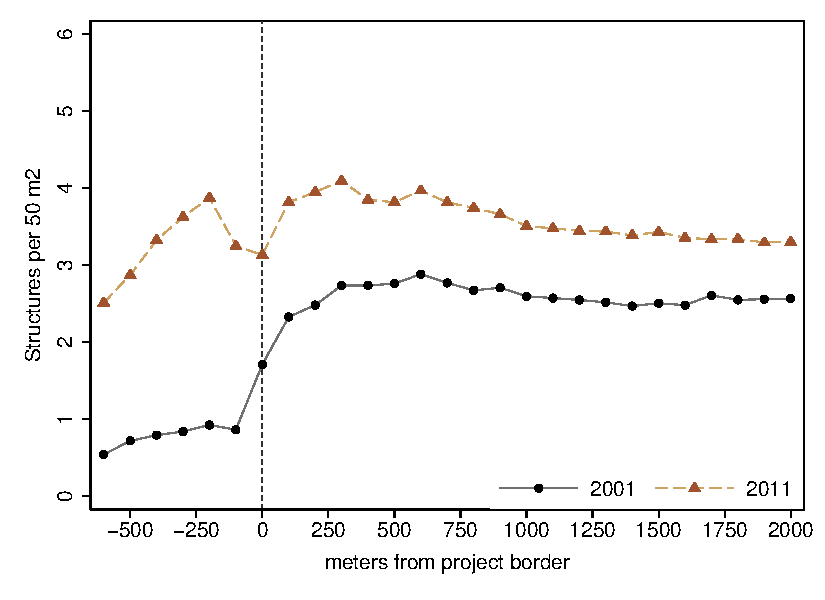
\includegraphics[scale=0.65,trim={5cm 1cm 5cm 0cm}]{figures/bblu/bblu_for_rdp_admin}
   \caption{formal structures, constructed projects.}
 \end{figure}
 \end{center}
}
\only<2>{
 \begin{center}
 \begin{figure}[ht]
   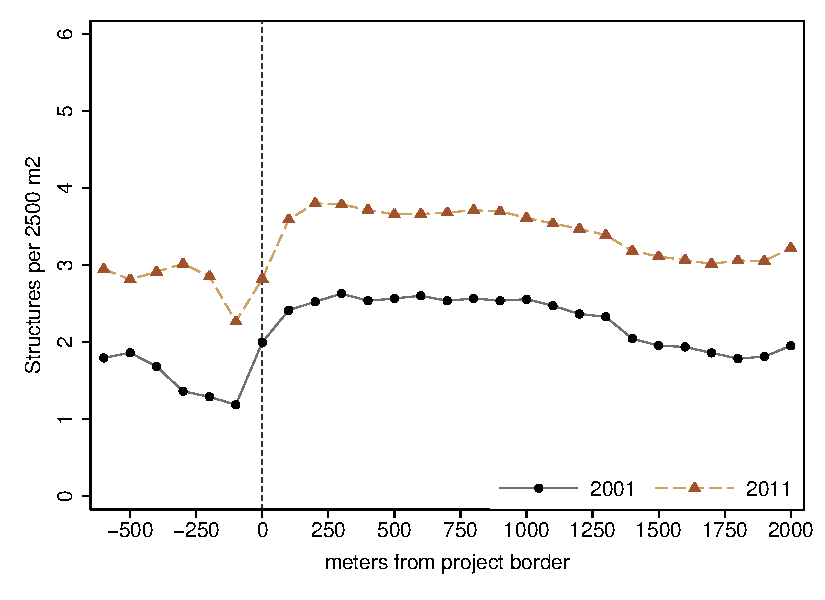
\includegraphics[scale=0.65,trim={5cm 1cm 5cm 0cm}]{figures/bblu/bblu_for_placebo_admin}
   \caption{formal structures, non-constructed projects.}
 \end{figure}
 \end{center}
}
\only<3>{
 \begin{center}
 \begin{figure}[ht]
   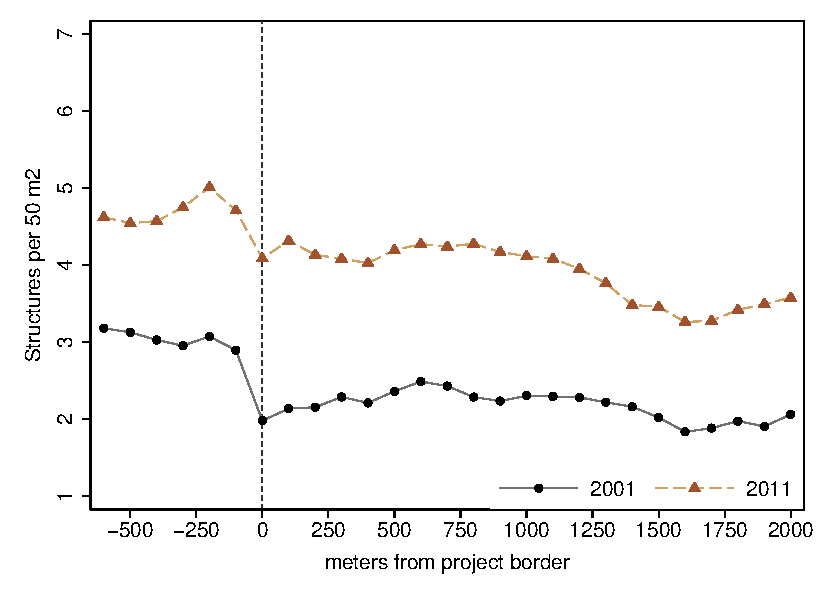
\includegraphics[scale=0.65,trim={5cm 1cm 5cm 0cm}]{figures/bblu/bblu_inf_rdp_admin}
   \caption{informal structures, constructed projects.}
 \end{figure}
 \end{center}
}
\only<4>{
 \begin{center}
 \begin{figure}[ht]
   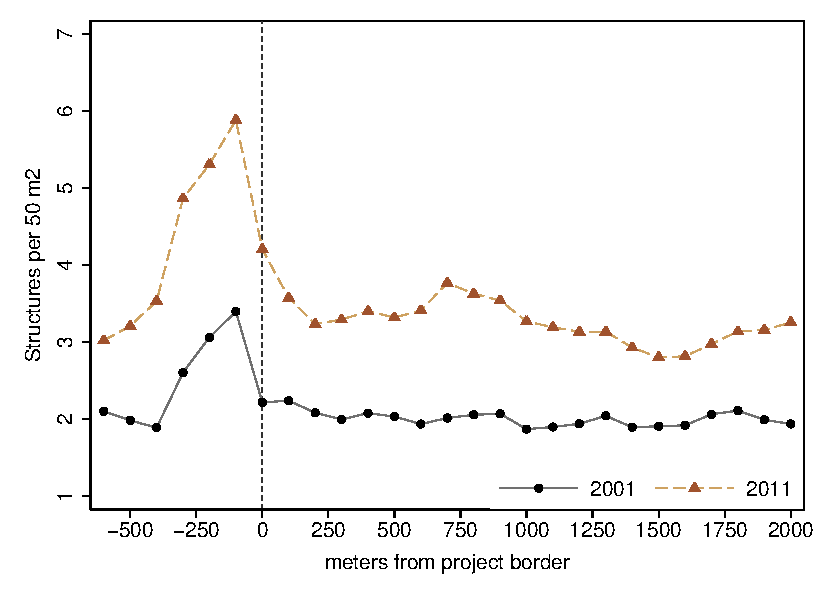
\includegraphics[scale=0.65,trim={5cm 1cm 5cm 0cm}]{figures/bblu/bblu_inf_placebo_admin}
   \caption{informal structures, non-constructed projects.}
 \end{figure}
 \end{center}
}
\end{frame}
%------------------------------------------------

\begin{frame}
\frametitle{Empirical Specification}

\begin{equation*}
y_{ipt} \, = \, \lambda_i + \sum\limits_{d} I^d_{ipt}\Big( \alpha^d D_tC_p \, + \, \beta^dD_t\Big) \, + \, \varepsilon_{ipt}
\end{equation*}
\only<1>{
\\with:
\begin{itemize}
\item $y_{itdp}$: building density for cell $i$ in vicinity of project $p$ observed in year $t$.
\item $I^d_{ip}$\,=1 if cell $i$ is at distance $d$ of project $p$.
\item $D_{t}\,\,$=1 if year $t$ is 2011 (post period). 
\item $C_{p}\,\,$=1 if project $p$ has been constructed.
\item $\lambda_i$: cell fixed-effect.
\item $\varepsilon_{itp}$: error term
\end{itemize}
}
\only<2>{
{\\\bf Density Outcomes:}
\begin{itemize}
\item total buildings.
\item formal buildings.
\item informal buildings.
\item backyard/non-backyard informal.
\end{itemize}
}
\end{frame}

%------------------------------------------------

\begin{frame}
\frametitle{Building Density: Estimation Results}
\only<1>{
 \begin{center}
 \begin{figure}[ht]
   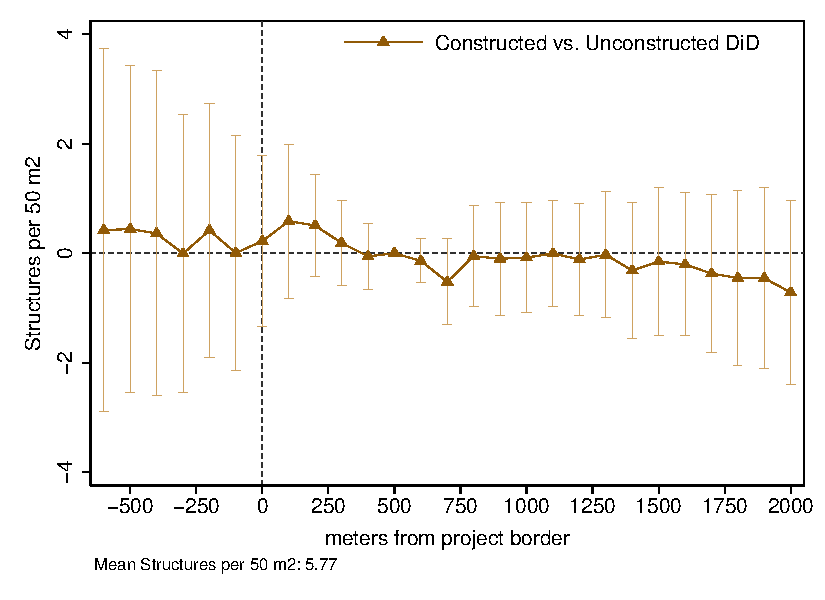
\includegraphics[scale=0.65,trim={5cm 1cm 5cm 0cm}]{figures/bblu/distplotDDD_bblu_total_buildings_admin}
   \caption{total structures}
 \end{figure}
 \end{center}
}
\only<2>{
 \begin{center}
 \begin{figure}[ht]
   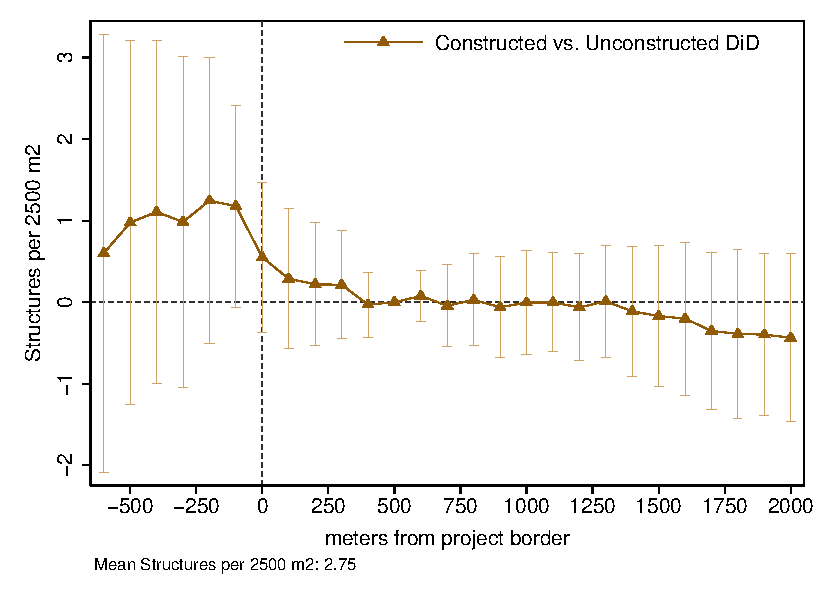
\includegraphics[scale=0.65,trim={5cm 1cm 5cm 0cm}]{figures/bblu/distplotDDD_bblu_for_admin}
   \caption{formal structures}
 \end{figure}
 \end{center}
}
\only<3>{
 \begin{center}
 \begin{figure}[ht]
   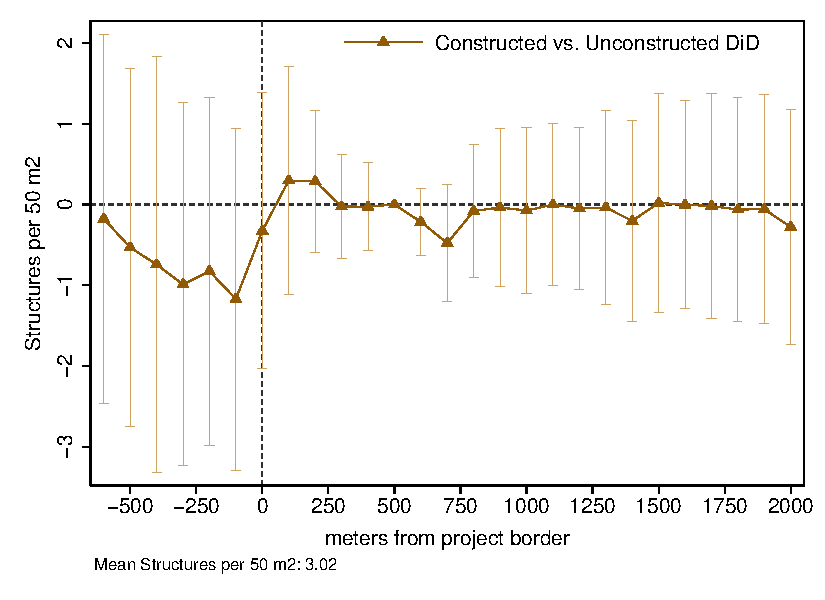
\includegraphics[scale=0.65,trim={5cm 1cm 5cm 0cm}]{figures/bblu/distplotDDD_bblu_inf_admin}
   \caption{informal structures}
 \end{figure}
 \end{center}
}
\only<4>{
 \begin{center}
 \begin{figure}[ht]
   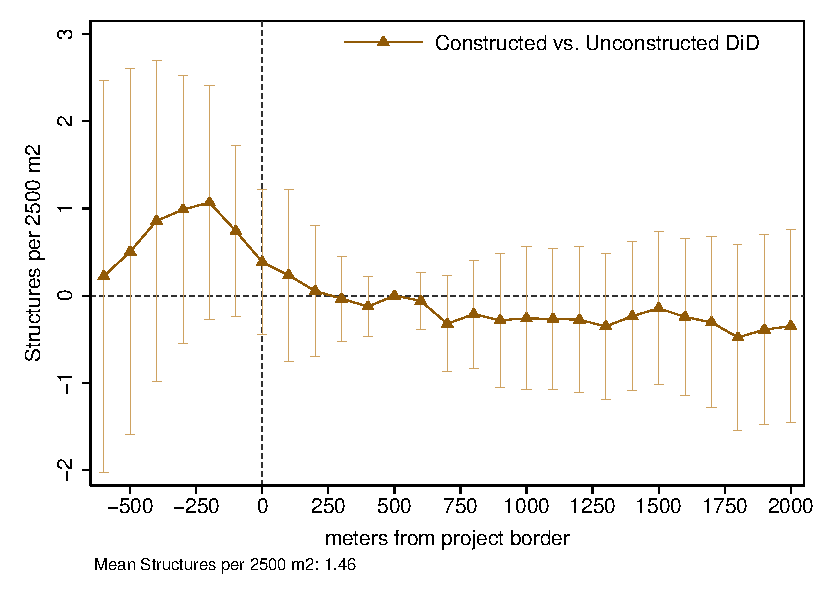
\includegraphics[scale=0.65,trim={5cm 1cm 5cm 0cm}]{figures/bblu/distplotDDD_bblu_inf_backyard_admin}
   \caption{informal backyard structures}
 \end{figure}
 \end{center}
}
\only<5>{
 \begin{center}
 \begin{figure}[ht]
   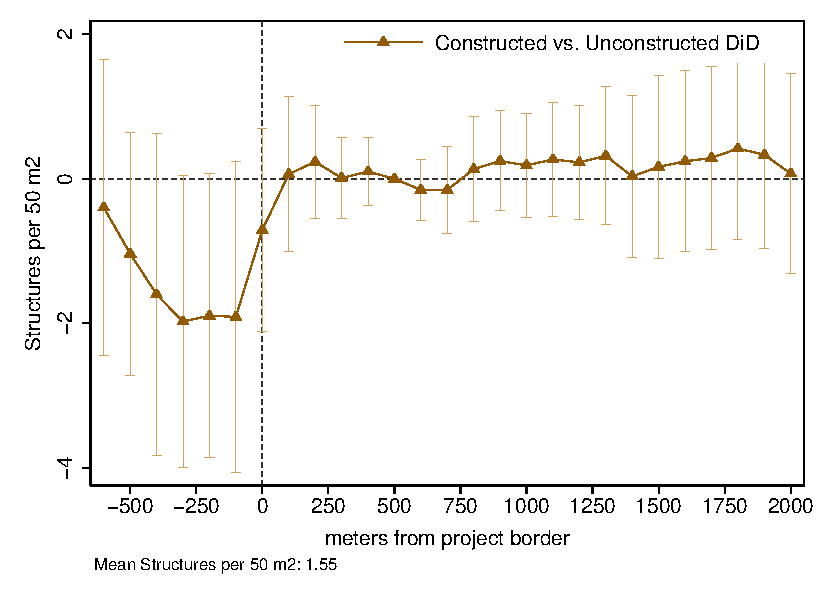
\includegraphics[scale=0.65,trim={5cm 1cm 5cm 0cm}]{figures/bblu/distplotDDD_bblu_inf_non_backyard_admin}
   \caption{informal non-backyard structures}
 \end{figure}
 \end{center}
}

\end{frame}

%------------------------------------------------

\begin{frame}
\frametitle{Triple Differences Tests}
\vspace{-1.5mm}
\begin{table}
-400m to 0m &      121.01   &      504.38** &     -383.37   &      419.94** &     -803.31***\\
            &    (296.06)   &    (206.69)   &    (292.55)   &    (181.72)   &    (265.47)   \\[0.5em]
0m to 400m  &      123.01   &       53.77   &       69.24   &       54.40   &       14.83   \\
            &    (148.32)   &    (104.60)   &    (148.03)   &    (130.97)   &    (114.79)   \\ \midrule
Mean dep. var.&    2,372.89   &    1,102.77   &    1,270.11   &      597.04   &      673.07   \\
\# Projects &         111   &         111   &         111   &         111   &         111   \\
R$^2$       &       0.098   &       0.116   &       0.055   &       0.101   &       0.044   \\
N           &     244,312   &     244,312   &     244,312   &     244,312   &     244,312   \\

\end{table}
\end{frame}

%------------------------------------------------

\section{Spillovers on Housing Prices}

%------------------------------------------------

\begin{frame}
\frametitle{Empirical Set-up}
\vspace{-1.5mm}
\begin{itemize}
\item Sample composed of non-subsidized formal housing transactions outside of project borders. 
\vspace{.5em}
\item Exact transaction date is observed.
\vspace{.5em}
\item Assign event date to {\bf constructed} projects.
\begin{itemize}
  \item modal transaction month for subsidized transactions.
\end{itemize}
\vspace{.5em}
\item Assign "event date" to {\bf unconstructed} projects.
\begin{itemize}
  \item apply average delay between project announcement and delivery.
\end{itemize}
\end{itemize}
\end{frame}

%------------------------------------------------

\begin{frame}
\frametitle{Transaction Densities}
\begin{center}
\begin{figure}
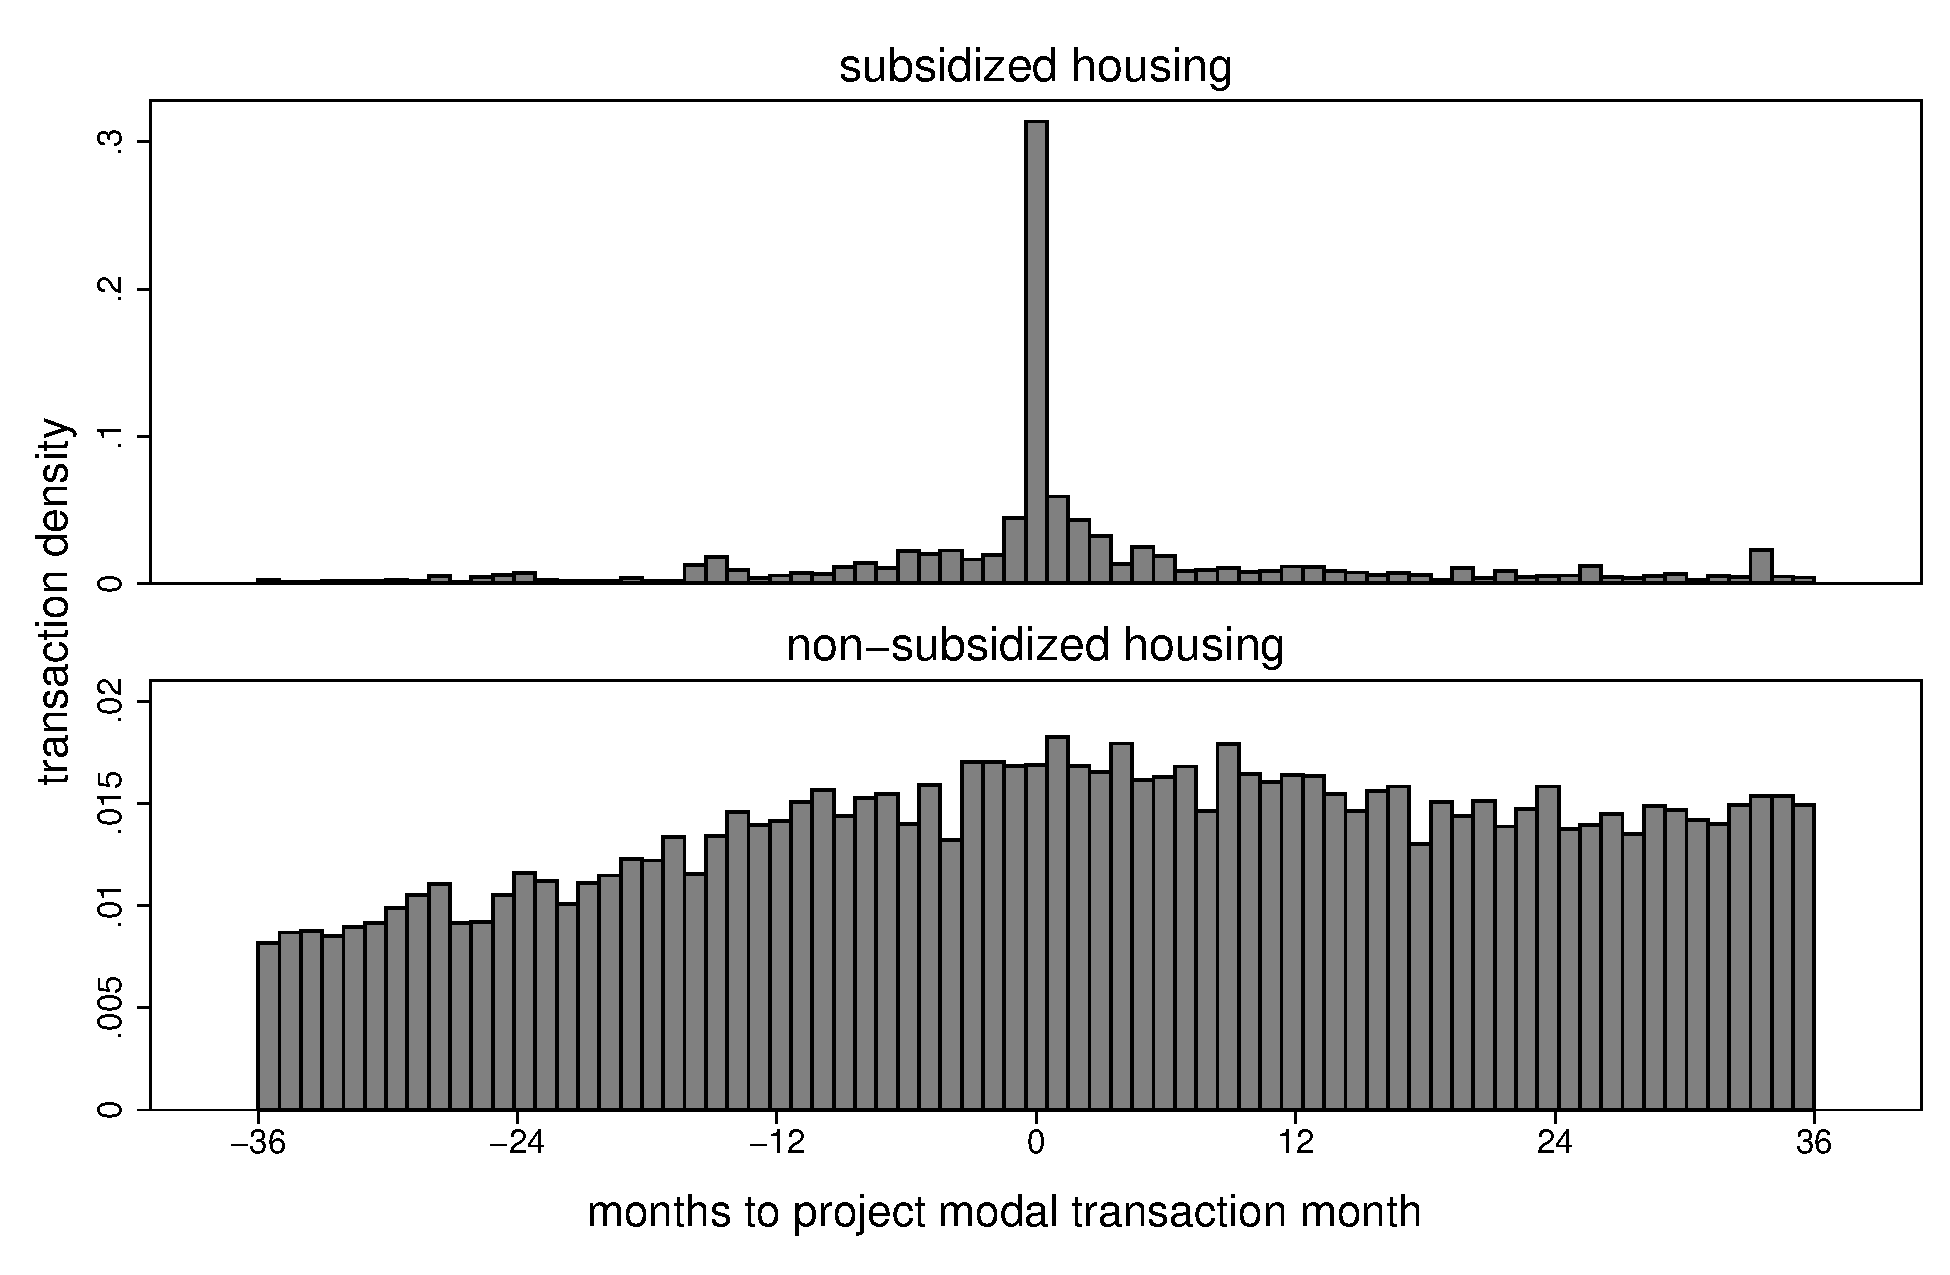
\includegraphics[scale=0.32]{figures/summary_densitytime.pdf}
\vspace{-3mm}
\end{figure}
\end{center}
\end{frame}

%------------------------------------------------

\begin{frame}
\frametitle{Empirical Specifications}
DID model:
\begin{equation*}
P_{itp} \, = \, \alpha D_{tp}T_{ip} \, + \,\theta_1 D_{tp} \, + \, \,\theta_2 T_{ip}+ \, X^{'}_{i}\beta \, +  \lambda_p \,  + \, \eta_{t} \, + \, \varepsilon_{itp} ,
\end{equation*}
with:
\begin{itemize}
\item $P_{itp}$: log-price of property $i$ sold at time $t$, in vicinity of project $p$.
\item $D_{tp}$ =1 if date $t$ is after modal construction month. 
\item $T_{ip}\,\,$ =1 if property $i$ within 700m of project border.
\item $X_{i}$: quadratic in lot size of property $i$.
\item $\lambda_p$: project fixed-effect.
\item $\eta_{t}$: time (year$\,\times\,$month) fixed-effect.

\item $\varepsilon_{itp}$: error term
\end{itemize}
\end{frame}

%------------------------------------------------

\begin{frame}
\frametitle{Housing Prices: Estimation Results}
\only<1>{
 \begin{center}
 \begin{figure}[ht]
   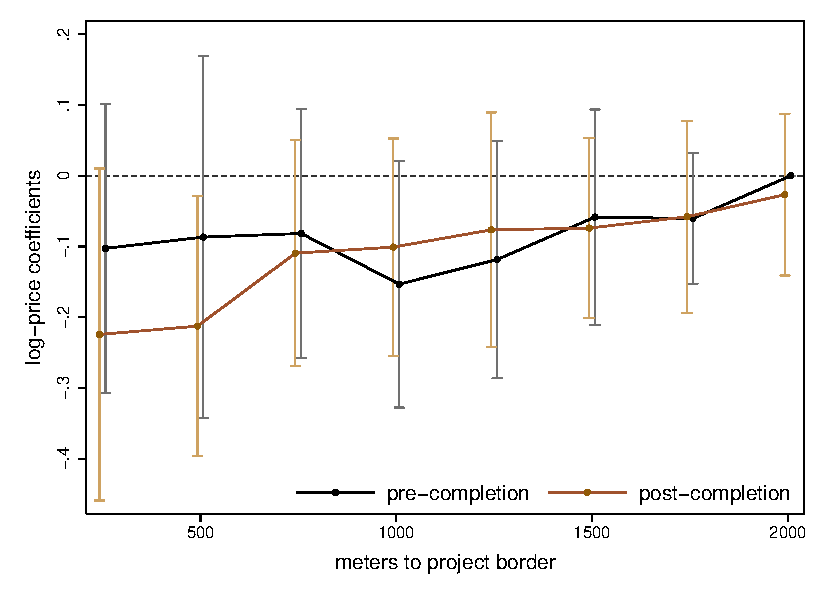
\includegraphics[scale=0.65,trim={5cm 1cm 5cm 0cm}]{figures/gradplot/distance_plot_rdp}
   \caption{proximity effects: constructed projects}
 \end{figure}
 \end{center}
}
\only<2>{
 \begin{center}
 \begin{figure}[ht]
   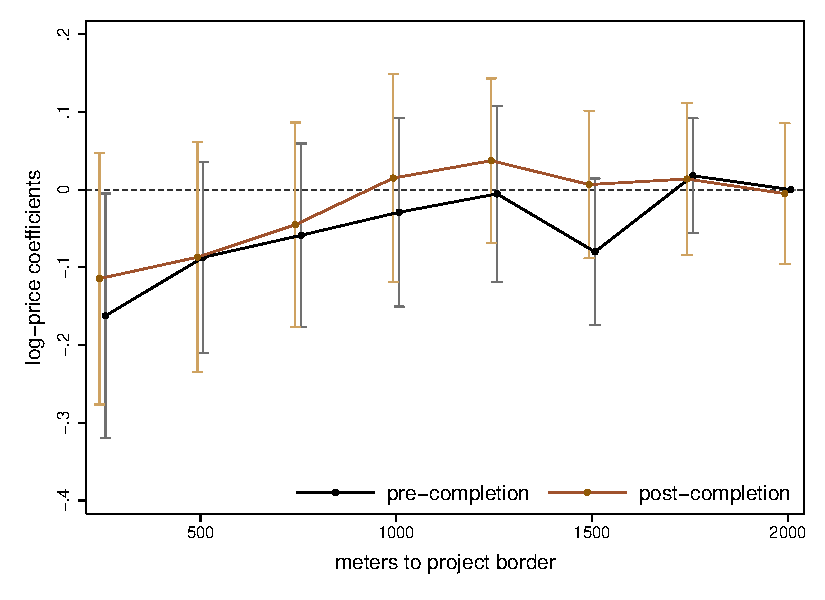
\includegraphics[scale=0.65,trim={5cm 1cm 5cm 0cm}]{figures/gradplot/distance_plot_placebo}
   \caption{proximity effects: non-constructed projects}
 \end{figure}
 \end{center}
}
\only<3>{
 \begin{center}
 \begin{figure}[ht]
   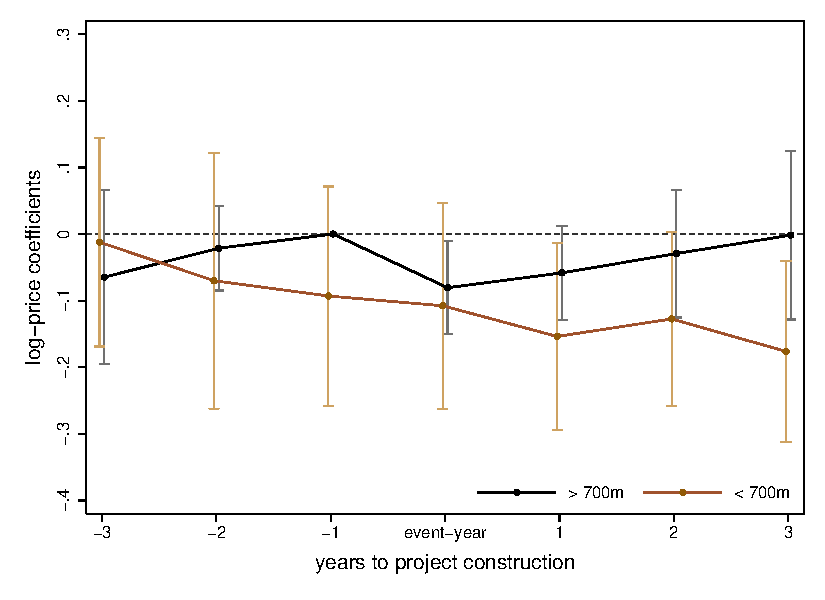
\includegraphics[scale=0.65,trim={5cm 1cm 5cm 0cm}]{figures/gradplot/time_plot_rdp}
   \caption{timing effects: constructed projects}
 \end{figure}
 \end{center}
}
\only<4>{
 \begin{center}
 \begin{figure}[ht]
   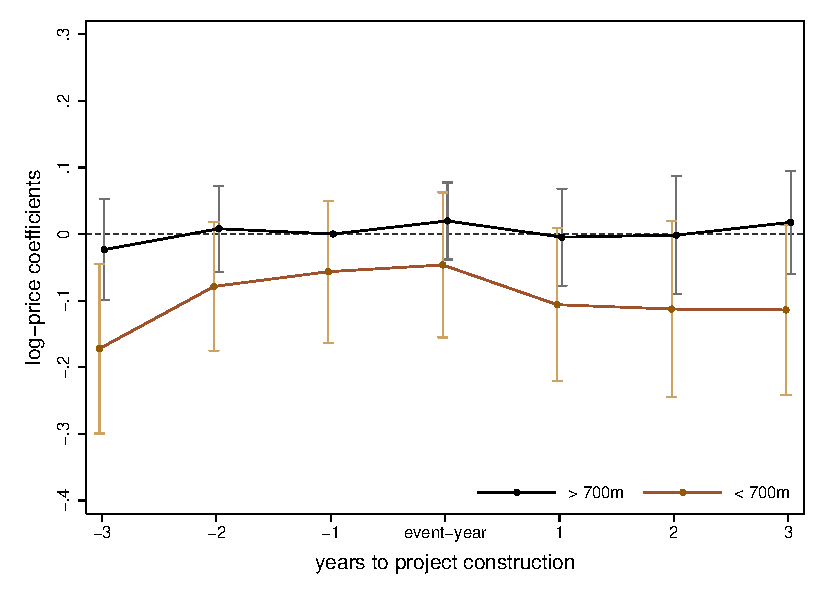
\includegraphics[scale=0.65,trim={5cm 1cm 5cm 0cm}]{figures/gradplot/time_plot_placebo}
   \caption{timing effects: non-constructed projects}
 \end{figure}
 \end{center}
}
\end{frame}

%------------------------------------------------


\end{document} 
